
\documentclass{article} % For LaTeX2e
\usepackage{iclr2025_conference,times}

% Optional math commands from https://github.com/goodfeli/dlbook_notation.
%%%%% NEW MATH DEFINITIONS %%%%%

\usepackage{amsmath,amsfonts,bm}
\usepackage{derivative}
% Mark sections of captions for referring to divisions of figures
\newcommand{\figleft}{{\em (Left)}}
\newcommand{\figcenter}{{\em (Center)}}
\newcommand{\figright}{{\em (Right)}}
\newcommand{\figtop}{{\em (Top)}}
\newcommand{\figbottom}{{\em (Bottom)}}
\newcommand{\captiona}{{\em (a)}}
\newcommand{\captionb}{{\em (b)}}
\newcommand{\captionc}{{\em (c)}}
\newcommand{\captiond}{{\em (d)}}

% Highlight a newly defined term
\newcommand{\newterm}[1]{{\bf #1}}

% Derivative d 
\newcommand{\deriv}{{\mathrm{d}}}

% Figure reference, lower-case.
\def\figref#1{figure~\ref{#1}}
% Figure reference, capital. For start of sentence
\def\Figref#1{Figure~\ref{#1}}
\def\twofigref#1#2{figures \ref{#1} and \ref{#2}}
\def\quadfigref#1#2#3#4{figures \ref{#1}, \ref{#2}, \ref{#3} and \ref{#4}}
% Section reference, lower-case.
\def\secref#1{section~\ref{#1}}
% Section reference, capital.
\def\Secref#1{Section~\ref{#1}}
% Reference to two sections.
\def\twosecrefs#1#2{sections \ref{#1} and \ref{#2}}
% Reference to three sections.
\def\secrefs#1#2#3{sections \ref{#1}, \ref{#2} and \ref{#3}}
% Reference to an equation, lower-case.
\def\eqref#1{equation~\ref{#1}}
% Reference to an equation, upper case
\def\Eqref#1{Equation~\ref{#1}}
% A raw reference to an equation---avoid using if possible
\def\plaineqref#1{\ref{#1}}
% Reference to a chapter, lower-case.
\def\chapref#1{chapter~\ref{#1}}
% Reference to an equation, upper case.
\def\Chapref#1{Chapter~\ref{#1}}
% Reference to a range of chapters
\def\rangechapref#1#2{chapters\ref{#1}--\ref{#2}}
% Reference to an algorithm, lower-case.
\def\algref#1{algorithm~\ref{#1}}
% Reference to an algorithm, upper case.
\def\Algref#1{Algorithm~\ref{#1}}
\def\twoalgref#1#2{algorithms \ref{#1} and \ref{#2}}
\def\Twoalgref#1#2{Algorithms \ref{#1} and \ref{#2}}
% Reference to a part, lower case
\def\partref#1{part~\ref{#1}}
% Reference to a part, upper case
\def\Partref#1{Part~\ref{#1}}
\def\twopartref#1#2{parts \ref{#1} and \ref{#2}}

\def\ceil#1{\lceil #1 \rceil}
\def\floor#1{\lfloor #1 \rfloor}
\def\1{\bm{1}}
\newcommand{\train}{\mathcal{D}}
\newcommand{\valid}{\mathcal{D_{\mathrm{valid}}}}
\newcommand{\test}{\mathcal{D_{\mathrm{test}}}}

\def\eps{{\epsilon}}


% Random variables
\def\reta{{\textnormal{$\eta$}}}
\def\ra{{\textnormal{a}}}
\def\rb{{\textnormal{b}}}
\def\rc{{\textnormal{c}}}
\def\rd{{\textnormal{d}}}
\def\re{{\textnormal{e}}}
\def\rf{{\textnormal{f}}}
\def\rg{{\textnormal{g}}}
\def\rh{{\textnormal{h}}}
\def\ri{{\textnormal{i}}}
\def\rj{{\textnormal{j}}}
\def\rk{{\textnormal{k}}}
\def\rl{{\textnormal{l}}}
% rm is already a command, just don't name any random variables m
\def\rn{{\textnormal{n}}}
\def\ro{{\textnormal{o}}}
\def\rp{{\textnormal{p}}}
\def\rq{{\textnormal{q}}}
\def\rr{{\textnormal{r}}}
\def\rs{{\textnormal{s}}}
\def\rt{{\textnormal{t}}}
\def\ru{{\textnormal{u}}}
\def\rv{{\textnormal{v}}}
\def\rw{{\textnormal{w}}}
\def\rx{{\textnormal{x}}}
\def\ry{{\textnormal{y}}}
\def\rz{{\textnormal{z}}}

% Random vectors
\def\rvepsilon{{\mathbf{\epsilon}}}
\def\rvphi{{\mathbf{\phi}}}
\def\rvtheta{{\mathbf{\theta}}}
\def\rva{{\mathbf{a}}}
\def\rvb{{\mathbf{b}}}
\def\rvc{{\mathbf{c}}}
\def\rvd{{\mathbf{d}}}
\def\rve{{\mathbf{e}}}
\def\rvf{{\mathbf{f}}}
\def\rvg{{\mathbf{g}}}
\def\rvh{{\mathbf{h}}}
\def\rvu{{\mathbf{i}}}
\def\rvj{{\mathbf{j}}}
\def\rvk{{\mathbf{k}}}
\def\rvl{{\mathbf{l}}}
\def\rvm{{\mathbf{m}}}
\def\rvn{{\mathbf{n}}}
\def\rvo{{\mathbf{o}}}
\def\rvp{{\mathbf{p}}}
\def\rvq{{\mathbf{q}}}
\def\rvr{{\mathbf{r}}}
\def\rvs{{\mathbf{s}}}
\def\rvt{{\mathbf{t}}}
\def\rvu{{\mathbf{u}}}
\def\rvv{{\mathbf{v}}}
\def\rvw{{\mathbf{w}}}
\def\rvx{{\mathbf{x}}}
\def\rvy{{\mathbf{y}}}
\def\rvz{{\mathbf{z}}}

% Elements of random vectors
\def\erva{{\textnormal{a}}}
\def\ervb{{\textnormal{b}}}
\def\ervc{{\textnormal{c}}}
\def\ervd{{\textnormal{d}}}
\def\erve{{\textnormal{e}}}
\def\ervf{{\textnormal{f}}}
\def\ervg{{\textnormal{g}}}
\def\ervh{{\textnormal{h}}}
\def\ervi{{\textnormal{i}}}
\def\ervj{{\textnormal{j}}}
\def\ervk{{\textnormal{k}}}
\def\ervl{{\textnormal{l}}}
\def\ervm{{\textnormal{m}}}
\def\ervn{{\textnormal{n}}}
\def\ervo{{\textnormal{o}}}
\def\ervp{{\textnormal{p}}}
\def\ervq{{\textnormal{q}}}
\def\ervr{{\textnormal{r}}}
\def\ervs{{\textnormal{s}}}
\def\ervt{{\textnormal{t}}}
\def\ervu{{\textnormal{u}}}
\def\ervv{{\textnormal{v}}}
\def\ervw{{\textnormal{w}}}
\def\ervx{{\textnormal{x}}}
\def\ervy{{\textnormal{y}}}
\def\ervz{{\textnormal{z}}}

% Random matrices
\def\rmA{{\mathbf{A}}}
\def\rmB{{\mathbf{B}}}
\def\rmC{{\mathbf{C}}}
\def\rmD{{\mathbf{D}}}
\def\rmE{{\mathbf{E}}}
\def\rmF{{\mathbf{F}}}
\def\rmG{{\mathbf{G}}}
\def\rmH{{\mathbf{H}}}
\def\rmI{{\mathbf{I}}}
\def\rmJ{{\mathbf{J}}}
\def\rmK{{\mathbf{K}}}
\def\rmL{{\mathbf{L}}}
\def\rmM{{\mathbf{M}}}
\def\rmN{{\mathbf{N}}}
\def\rmO{{\mathbf{O}}}
\def\rmP{{\mathbf{P}}}
\def\rmQ{{\mathbf{Q}}}
\def\rmR{{\mathbf{R}}}
\def\rmS{{\mathbf{S}}}
\def\rmT{{\mathbf{T}}}
\def\rmU{{\mathbf{U}}}
\def\rmV{{\mathbf{V}}}
\def\rmW{{\mathbf{W}}}
\def\rmX{{\mathbf{X}}}
\def\rmY{{\mathbf{Y}}}
\def\rmZ{{\mathbf{Z}}}

% Elements of random matrices
\def\ermA{{\textnormal{A}}}
\def\ermB{{\textnormal{B}}}
\def\ermC{{\textnormal{C}}}
\def\ermD{{\textnormal{D}}}
\def\ermE{{\textnormal{E}}}
\def\ermF{{\textnormal{F}}}
\def\ermG{{\textnormal{G}}}
\def\ermH{{\textnormal{H}}}
\def\ermI{{\textnormal{I}}}
\def\ermJ{{\textnormal{J}}}
\def\ermK{{\textnormal{K}}}
\def\ermL{{\textnormal{L}}}
\def\ermM{{\textnormal{M}}}
\def\ermN{{\textnormal{N}}}
\def\ermO{{\textnormal{O}}}
\def\ermP{{\textnormal{P}}}
\def\ermQ{{\textnormal{Q}}}
\def\ermR{{\textnormal{R}}}
\def\ermS{{\textnormal{S}}}
\def\ermT{{\textnormal{T}}}
\def\ermU{{\textnormal{U}}}
\def\ermV{{\textnormal{V}}}
\def\ermW{{\textnormal{W}}}
\def\ermX{{\textnormal{X}}}
\def\ermY{{\textnormal{Y}}}
\def\ermZ{{\textnormal{Z}}}

% Vectors
\def\vzero{{\bm{0}}}
\def\vone{{\bm{1}}}
\def\vmu{{\bm{\mu}}}
\def\vtheta{{\bm{\theta}}}
\def\vphi{{\bm{\phi}}}
\def\va{{\bm{a}}}
\def\vb{{\bm{b}}}
\def\vc{{\bm{c}}}
\def\vd{{\bm{d}}}
\def\ve{{\bm{e}}}
\def\vf{{\bm{f}}}
\def\vg{{\bm{g}}}
\def\vh{{\bm{h}}}
\def\vi{{\bm{i}}}
\def\vj{{\bm{j}}}
\def\vk{{\bm{k}}}
\def\vl{{\bm{l}}}
\def\vm{{\bm{m}}}
\def\vn{{\bm{n}}}
\def\vo{{\bm{o}}}
\def\vp{{\bm{p}}}
\def\vq{{\bm{q}}}
\def\vr{{\bm{r}}}
\def\vs{{\bm{s}}}
\def\vt{{\bm{t}}}
\def\vu{{\bm{u}}}
\def\vv{{\bm{v}}}
\def\vw{{\bm{w}}}
\def\vx{{\bm{x}}}
\def\vy{{\bm{y}}}
\def\vz{{\bm{z}}}

% Elements of vectors
\def\evalpha{{\alpha}}
\def\evbeta{{\beta}}
\def\evepsilon{{\epsilon}}
\def\evlambda{{\lambda}}
\def\evomega{{\omega}}
\def\evmu{{\mu}}
\def\evpsi{{\psi}}
\def\evsigma{{\sigma}}
\def\evtheta{{\theta}}
\def\eva{{a}}
\def\evb{{b}}
\def\evc{{c}}
\def\evd{{d}}
\def\eve{{e}}
\def\evf{{f}}
\def\evg{{g}}
\def\evh{{h}}
\def\evi{{i}}
\def\evj{{j}}
\def\evk{{k}}
\def\evl{{l}}
\def\evm{{m}}
\def\evn{{n}}
\def\evo{{o}}
\def\evp{{p}}
\def\evq{{q}}
\def\evr{{r}}
\def\evs{{s}}
\def\evt{{t}}
\def\evu{{u}}
\def\evv{{v}}
\def\evw{{w}}
\def\evx{{x}}
\def\evy{{y}}
\def\evz{{z}}

% Matrix
\def\mA{{\bm{A}}}
\def\mB{{\bm{B}}}
\def\mC{{\bm{C}}}
\def\mD{{\bm{D}}}
\def\mE{{\bm{E}}}
\def\mF{{\bm{F}}}
\def\mG{{\bm{G}}}
\def\mH{{\bm{H}}}
\def\mI{{\bm{I}}}
\def\mJ{{\bm{J}}}
\def\mK{{\bm{K}}}
\def\mL{{\bm{L}}}
\def\mM{{\bm{M}}}
\def\mN{{\bm{N}}}
\def\mO{{\bm{O}}}
\def\mP{{\bm{P}}}
\def\mQ{{\bm{Q}}}
\def\mR{{\bm{R}}}
\def\mS{{\bm{S}}}
\def\mT{{\bm{T}}}
\def\mU{{\bm{U}}}
\def\mV{{\bm{V}}}
\def\mW{{\bm{W}}}
\def\mX{{\bm{X}}}
\def\mY{{\bm{Y}}}
\def\mZ{{\bm{Z}}}
\def\mBeta{{\bm{\beta}}}
\def\mPhi{{\bm{\Phi}}}
\def\mLambda{{\bm{\Lambda}}}
\def\mSigma{{\bm{\Sigma}}}

% Tensor
\DeclareMathAlphabet{\mathsfit}{\encodingdefault}{\sfdefault}{m}{sl}
\SetMathAlphabet{\mathsfit}{bold}{\encodingdefault}{\sfdefault}{bx}{n}
\newcommand{\tens}[1]{\bm{\mathsfit{#1}}}
\def\tA{{\tens{A}}}
\def\tB{{\tens{B}}}
\def\tC{{\tens{C}}}
\def\tD{{\tens{D}}}
\def\tE{{\tens{E}}}
\def\tF{{\tens{F}}}
\def\tG{{\tens{G}}}
\def\tH{{\tens{H}}}
\def\tI{{\tens{I}}}
\def\tJ{{\tens{J}}}
\def\tK{{\tens{K}}}
\def\tL{{\tens{L}}}
\def\tM{{\tens{M}}}
\def\tN{{\tens{N}}}
\def\tO{{\tens{O}}}
\def\tP{{\tens{P}}}
\def\tQ{{\tens{Q}}}
\def\tR{{\tens{R}}}
\def\tS{{\tens{S}}}
\def\tT{{\tens{T}}}
\def\tU{{\tens{U}}}
\def\tV{{\tens{V}}}
\def\tW{{\tens{W}}}
\def\tX{{\tens{X}}}
\def\tY{{\tens{Y}}}
\def\tZ{{\tens{Z}}}


% Graph
\def\gA{{\mathcal{A}}}
\def\gB{{\mathcal{B}}}
\def\gC{{\mathcal{C}}}
\def\gD{{\mathcal{D}}}
\def\gE{{\mathcal{E}}}
\def\gF{{\mathcal{F}}}
\def\gG{{\mathcal{G}}}
\def\gH{{\mathcal{H}}}
\def\gI{{\mathcal{I}}}
\def\gJ{{\mathcal{J}}}
\def\gK{{\mathcal{K}}}
\def\gL{{\mathcal{L}}}
\def\gM{{\mathcal{M}}}
\def\gN{{\mathcal{N}}}
\def\gO{{\mathcal{O}}}
\def\gP{{\mathcal{P}}}
\def\gQ{{\mathcal{Q}}}
\def\gR{{\mathcal{R}}}
\def\gS{{\mathcal{S}}}
\def\gT{{\mathcal{T}}}
\def\gU{{\mathcal{U}}}
\def\gV{{\mathcal{V}}}
\def\gW{{\mathcal{W}}}
\def\gX{{\mathcal{X}}}
\def\gY{{\mathcal{Y}}}
\def\gZ{{\mathcal{Z}}}

% Sets
\def\sA{{\mathbb{A}}}
\def\sB{{\mathbb{B}}}
\def\sC{{\mathbb{C}}}
\def\sD{{\mathbb{D}}}
% Don't use a set called E, because this would be the same as our symbol
% for expectation.
\def\sF{{\mathbb{F}}}
\def\sG{{\mathbb{G}}}
\def\sH{{\mathbb{H}}}
\def\sI{{\mathbb{I}}}
\def\sJ{{\mathbb{J}}}
\def\sK{{\mathbb{K}}}
\def\sL{{\mathbb{L}}}
\def\sM{{\mathbb{M}}}
\def\sN{{\mathbb{N}}}
\def\sO{{\mathbb{O}}}
\def\sP{{\mathbb{P}}}
\def\sQ{{\mathbb{Q}}}
\def\sR{{\mathbb{R}}}
\def\sS{{\mathbb{S}}}
\def\sT{{\mathbb{T}}}
\def\sU{{\mathbb{U}}}
\def\sV{{\mathbb{V}}}
\def\sW{{\mathbb{W}}}
\def\sX{{\mathbb{X}}}
\def\sY{{\mathbb{Y}}}
\def\sZ{{\mathbb{Z}}}

% Entries of a matrix
\def\emLambda{{\Lambda}}
\def\emA{{A}}
\def\emB{{B}}
\def\emC{{C}}
\def\emD{{D}}
\def\emE{{E}}
\def\emF{{F}}
\def\emG{{G}}
\def\emH{{H}}
\def\emI{{I}}
\def\emJ{{J}}
\def\emK{{K}}
\def\emL{{L}}
\def\emM{{M}}
\def\emN{{N}}
\def\emO{{O}}
\def\emP{{P}}
\def\emQ{{Q}}
\def\emR{{R}}
\def\emS{{S}}
\def\emT{{T}}
\def\emU{{U}}
\def\emV{{V}}
\def\emW{{W}}
\def\emX{{X}}
\def\emY{{Y}}
\def\emZ{{Z}}
\def\emSigma{{\Sigma}}

% entries of a tensor
% Same font as tensor, without \bm wrapper
\newcommand{\etens}[1]{\mathsfit{#1}}
\def\etLambda{{\etens{\Lambda}}}
\def\etA{{\etens{A}}}
\def\etB{{\etens{B}}}
\def\etC{{\etens{C}}}
\def\etD{{\etens{D}}}
\def\etE{{\etens{E}}}
\def\etF{{\etens{F}}}
\def\etG{{\etens{G}}}
\def\etH{{\etens{H}}}
\def\etI{{\etens{I}}}
\def\etJ{{\etens{J}}}
\def\etK{{\etens{K}}}
\def\etL{{\etens{L}}}
\def\etM{{\etens{M}}}
\def\etN{{\etens{N}}}
\def\etO{{\etens{O}}}
\def\etP{{\etens{P}}}
\def\etQ{{\etens{Q}}}
\def\etR{{\etens{R}}}
\def\etS{{\etens{S}}}
\def\etT{{\etens{T}}}
\def\etU{{\etens{U}}}
\def\etV{{\etens{V}}}
\def\etW{{\etens{W}}}
\def\etX{{\etens{X}}}
\def\etY{{\etens{Y}}}
\def\etZ{{\etens{Z}}}

% The true underlying data generating distribution
\newcommand{\pdata}{p_{\rm{data}}}
\newcommand{\ptarget}{p_{\rm{target}}}
\newcommand{\pprior}{p_{\rm{prior}}}
\newcommand{\pbase}{p_{\rm{base}}}
\newcommand{\pref}{p_{\rm{ref}}}

% The empirical distribution defined by the training set
\newcommand{\ptrain}{\hat{p}_{\rm{data}}}
\newcommand{\Ptrain}{\hat{P}_{\rm{data}}}
% The model distribution
\newcommand{\pmodel}{p_{\rm{model}}}
\newcommand{\Pmodel}{P_{\rm{model}}}
\newcommand{\ptildemodel}{\tilde{p}_{\rm{model}}}
% Stochastic autoencoder distributions
\newcommand{\pencode}{p_{\rm{encoder}}}
\newcommand{\pdecode}{p_{\rm{decoder}}}
\newcommand{\precons}{p_{\rm{reconstruct}}}

\newcommand{\laplace}{\mathrm{Laplace}} % Laplace distribution

\newcommand{\E}{\mathbb{E}}
\newcommand{\Ls}{\mathcal{L}}
\newcommand{\R}{\mathbb{R}}
\newcommand{\emp}{\tilde{p}}
\newcommand{\lr}{\alpha}
\newcommand{\reg}{\lambda}
\newcommand{\rect}{\mathrm{rectifier}}
\newcommand{\softmax}{\mathrm{softmax}}
\newcommand{\sigmoid}{\sigma}
\newcommand{\softplus}{\zeta}
\newcommand{\KL}{D_{\mathrm{KL}}}
\newcommand{\Var}{\mathrm{Var}}
\newcommand{\standarderror}{\mathrm{SE}}
\newcommand{\Cov}{\mathrm{Cov}}
% Wolfram Mathworld says $L^2$ is for function spaces and $\ell^2$ is for vectors
% But then they seem to use $L^2$ for vectors throughout the site, and so does
% wikipedia.
\newcommand{\normlzero}{L^0}
\newcommand{\normlone}{L^1}
\newcommand{\normltwo}{L^2}
\newcommand{\normlp}{L^p}
\newcommand{\normmax}{L^\infty}

\newcommand{\parents}{Pa} % See usage in notation.tex. Chosen to match Daphne's book.

\DeclareMathOperator*{\argmax}{arg\,max}
\DeclareMathOperator*{\argmin}{arg\,min}

\DeclareMathOperator{\sign}{sign}
\DeclareMathOperator{\Tr}{Tr}
\let\ab\allowbreak


\usepackage{hyperref}
\usepackage{url}
\usepackage{multirow}
\usepackage{tikz}
\usepackage{multicol}
\usepackage{graphicx}
\usepackage{booktabs}

\usepackage{tikz}
\usepackage{multirow}
\usepackage{xcolor}
\usepackage{pgfplots}
\usepackage{pgfplotstable}
\pgfplotsset{compat=newest}
\usepackage{amsmath}
\usepackage{amssymb}
\usetikzlibrary{positioning,shapes,arrows,shadows,patterns}
\usepackage{subfig}
% \usepackage{subfigure}
% \usepackage{subcaption}
\usepackage{caption}
\usepackage{soul}
\usepackage{ragged2e}

\newcommand{\revised}[1]{{\color{blue}#1}}

\usepackage{enumitem}
\newcommand{\basicalert}[2]{\fbox{\bfseries\sffamily\scriptsize\color{red} #1}{\sf\small$\blacktriangleright$\textit{\color{blue} #2}$\blacktriangleleft$}}
\newcommand{\bei}[1]{\basicalert{From Bei}{#1}}
\newcommand{\gangao}[1]{\basicalert{From Gangao Liu}{#1}}
\newcommand{\src}[1]{\basicalert{From SRC}{#1}}
\newcommand{\cy}[1]{\basicalert{From Chen Yang}{#1}}

\definecolor{citecolor}{HTML}{0071BC}
\definecolor{linkcolor}{HTML}{ED1C24}
\hypersetup{pagebackref=true, breaklinks=true, letterpaper=true,colorlinks=true, citecolor=citecolor, linkcolor=linkcolor, urlcolor=purple, bookmarksopen=true, bookmarksopenlevel=2, bookmarksnumbered=true} % hyperlinks


\newcommand{\method}{$\textrm{D}^2\textrm{PO}$ }


\usepackage{wrapfig}
% \usepackage{warptable}

\title{Earlier Tokens Contribute More: Learning Direct Preference Optimization From Temporal Decay Perspective}

% Authors must not appear in the submitted version. They should be hidden
% as long as the \iclrfinalcopy macro remains commented out below.
% Non-anonymous submissions will be rejected without review.

\author{%
  Ruichen Shao${}^{1}\thanks{Equal Contributions.}$ \ \ \ \ Bei Li${}^{1*}\thanks{Corresponding Author.}$ \ \ \ \  Gangao Liu${}^{2}$ \ \ \ \ Yang Chen${}^1$ \ \ \ \ Xiang Zhou${}^1$ \\ \textbf{Jingang Wang}${}^{1\dag}$ \ \ \ \ \textbf{Xunliang Cai}${}^1$ \ \ \ \ \textbf{Peng Li}${}^2$ \\ 
  ${}^1$Meituan Inc. \ \ \ \ ${}^2$University of Chinese Academy of Sciences \ \ \ \  \\ 
\texttt{\{shaoruichen,libei17,chenyang108,wangjingang02\}@meituan.com} \\
\texttt{\{liugangao2023,lipeng\}@iscas.ac.cn}}


% The \author macro works with any number of authors. There are two commands
% used to separate the names and addresses of multiple authors: \And and \AND.
%
% Using \And between authors leaves it to \LaTeX{} to determine where to break
% the lines. Using \AND forces a linebreak at that point. So, if \LaTeX{}
% puts 3 of 4 authors names on the first line, and the last on the second
% line, try using \AND instead of \And before the third author name.

\newcommand{\fix}{\marginpar{FIX}}
\newcommand{\new}{\marginpar{NEW}}

\iclrfinalcopy
% Uncomment for camera-ready version, but NOT for submission.
\begin{document}


\maketitle

\begin{abstract}
Direct Preference Optimization (DPO) has gained attention as an efficient alternative to reinforcement learning from human feedback (RLHF) for aligning large language models (LLMs) with human preferences. Despite its advantages, DPO suffers from a length bias, generating responses longer than those from the reference model. Existing solutions like SimPO and SamPO address this issue but uniformly treat the contribution of rewards across sequences, overlooking temporal dynamics. To this end, we propose an enhanced preference optimization method that incorporates a temporal decay factor controlled by a gamma parameter. This dynamic weighting mechanism adjusts the influence of each reward based on its position in the sequence, prioritizing earlier tokens that are more critical for alignment. By adaptively focusing on more relevant feedback, our approach mitigates overfitting to less pertinent data and remains responsive to evolving human preferences. Experimental results on several benchmarks show that our approach consistently outperforms vanilla DPO by 5.9-8.8 points on AlpacaEval 2 and 3.3-9.7 points on Arena-Hard across different model architectures and sizes. 
Furthermore, additional experiments on mathematical and reasoning benchmarks (MMLU, GSM8K, and MATH) confirm that our method enhances performance without compromising general capabilities. Our codebase would be available at \url{https://github.com/LotuSrc/D2PO}.

\end{abstract}



\section{Introduction}

Direct Preference Optimization (DPO)~\citep{Rafailov2023DirectPO} has recently emerged as a highly efficient alternative for aligning large language models (LLMs) with human preferences ~\citep{Askell2021AGL, Ouyang2022TrainingLM}. Unlike reinforcement learning from human feedback (RLHF), which involves training a reward model followed by iterative policy updates, DPO reframes the problem as a binary classification task directly over human preference data. 
Compared to supervised fine-tuning, DPO enables the model not only to learn what is good but also to be aware of what is bad.
This formulation allows DPO to optimize preference alignment in a single-stage training process, bypassing the complexities of reinforcement learning, such as policy sampling or extensive hyperparameter tuning. By leveraging an analytical mapping between reward functions and optimal policies, DPO fine-tunes LLMs efficiently and stably, offering superior performance in tasks like sentiment control, summarization, and dialogue generation while reducing computational overhead.

% Despite its advantages, DPO suffers from a length bias problem, which is caused by the unbalanced length preference due to the non-uniform length distribution of chosen and rejected responses. This leads to generated responses tending to be longer than those of the reference model if the majority of chosen responses are longer than the rejected ones. Several approaches have emerged to address this issue. One such method is SimPO~\citep{Meng2024SimPO}, which introduces a more streamlined framework by eliminating the need for a reference model. Instead of relying on a pre-trained reference model for comparison, SimPO uses the average log probability of a generated sequence as the implicit reward signal. This innovation reduces computational complexity and memory usage, making SimPO a more efficient alternative to DPO. However, our experiments have revealed that SimPO suffers from unexpected performance issues when applied to data not generated through self-sampling. Similarly, \citet{lu2024sampo} proposed SamPO to address the length bias inherent in DPO. By constraining the reward computation to the shorter time-series range between the chosen and rejected responses, SamPO mitigates biases arising from sequence length disparities, thereby refining the preference optimization process. 

Despite its advantages, DPO suffers from a length bias problem, which is caused by the unbalanced length preference due to the non-uniform length distribution of chosen and rejected responses. This leads to generated responses tending to be longer than those of the reference model if the majority of chosen responses are longer than the rejected ones. To address this, SimPO~\citep{Meng2024SimPO} introduces a more streamlined framework by eliminating the need for a reference model. Instead of relying on a pre-trained reference model for comparison, SimPO uses the average log probability of a generated sequence as the implicit reward signal. This innovation reduces computational complexity and memory usage, making SimPO a more efficient alternative to DPO. However, our experiments have revealed that SimPO suffers from unexpected performance issues when applied to data not generated through self-sampling. Similarly, SamPO~\citep{lu2024sampo} addresses DPO's length bias by limiting reward computation to the shorter time-series range between chosen and rejected responses, thereby the refining preference optimization.

%----------------------------------------------
\begin{wrapfigure}[17]{r}{6.5cm}
    \centering
    \vspace{-0.30cm}
    \begin{tikzpicture}
      \scriptsize{
      \begin{axis}[
      width=.48\textwidth, height=.32\textwidth ,
      xlabel=Response Position,
      ylabel=KL Divergence,
      xmin=0, xmax=1450,
      ymin=0, ymax=3.3,
      xtick={0,200,400,600,800,1000, 1200,1400},
      %xticklabels={$0$,$10$,$20$,$30$,$40$,$50$},
      ytick={0.5,1.0,1.5,2.0,2.5,3.0},
      % yticklabels={$0.1$,$0.2$,$0.3$,$0.4$,$0.5$,$0.6$},
      ymajorgrids=true,
      xmajorgrids=true,
      grid style=dashdotted,
      legend cell align=left,
      scaled ticks=false,
      xlabel style={align=center,font=\scriptsize},
      ylabel style={font=\scriptsize,yshift=0em},
      yticklabel style={/pgf/number format/fixed,/pgf/number format/fixed zerofill,/pgf/number format/precision=1},
      ytick style={opacity=0},
      legend style={yshift=-0.2em,xshift=0em,legend cell align=left,legend plot pos=right},
      ]
      \addplot [sharp plot,red,mark size=1pt,thick,line width=0.5pt,mark size=0.2pt] table [x=position,y=value,col sep=comma] {./Figure/llama_self_sampling.csv};
      \addplot [sharp plot,blue,mark size=1pt,thick,line width=0.5pt,mark size=0.2pt] table [x=position,y=value,col sep=comma] {./Figure/gemma_self_sampling.csv};
      \addplot [sharp plot,orange,mark size=1pt,thick,line width=0.5pt,smooth] table [x=position,y=value,col sep=comma] {Figure/mistral_self_sampling.csv};
      \legend{\tiny{Llama3-Instruct (8B)},\tiny{Gemma2-Instruct (9B)},\tiny{Mistral-NeMo-Instruct (12B)}},
      \end{axis}
      }
      \end{tikzpicture}
    \caption{Visualization of KL divergence of instruct models and their DPO variants. The results include three widely used open-source LLMs: Llama3, Gemma2, and Mistral-NeMo. Observation here indicates earlier tokens contribute more during alignment.}
     \label{fig:self_sampling}
    \end{wrapfigure}
  %----------------------------------------------




  %----------------------------------------------
% \begin{wrapfigure}[16]{r}{6.5cm}
%     \centering
%     \vspace{-0.0in}
%     \begin{tikzpicture}
%       \scriptsize{
%       \begin{axis}[
%       width=.48\textwidth, height=.32\textwidth ,
%       xlabel=Position,
%       ylabel=KL Divergence,
%       xmin=0, xmax=1050,
%       ymin=0, ymax=1.2,
%       xtick={0,200,400,600,800,1000},
%       %xticklabels={$0$,$10$,$20$,$30$,$40$,$50$},
%       ytick={0.2,0.4,...,1.4},
%       % yticklabels={$0.1$,$0.2$,$0.3$,$0.4$,$0.5$,$0.6$},
%       ymajorgrids=true,
%       xmajorgrids=true,
%       grid style=dashdotted,
%       legend cell align=left,
%       scaled ticks=false,
%       xlabel style={align=center,font=\scriptsize},
%       ylabel style={font=\scriptsize,yshift=0em},
%       yticklabel style={/pgf/number format/fixed,/pgf/number format/fixed zerofill,/pgf/number format/precision=1},
%       ytick style={opacity=0},
%       % xtick label style={font=\tiny},
%       % ytick label style={font=\tiny},
%       legend style={yshift=-0.2em,xshift=0em,legend cell align=left,legend plot pos=right},
%       ]
%       \addplot [sharp plot,red,mark size=1pt,thick,line width=0.5pt,mark size=0.2pt] table [x=position,y=value,col sep=comma] {./Figure/llama_self_target_kl.csv};
%       \addplot [sharp plot,blue,mark size=1pt,thick,line width=0.5pt,mark size=0.2pt] table [x=position,y=value,col sep=comma] {./Figure/gemma_self_target_kl.csv};
%       \addplot [sharp plot,orange,mark size=1pt,thick,line width=0.5pt,smooth] table [x=position,y=value,col sep=comma] {Figure/mistral_self_target_kl.csv};
%       \legend{\tiny{Llama3-Instruct (8B)},\tiny{Gemma2-Instruct (9B)},\tiny{Mistral-NeMo-Instruct (12B)}},
%       \end{axis}
%       }
%       \end{tikzpicture}
%     \caption{Visualization of the KL divergence of instruct models and their subsequent DPO variants. The results include three widely used open-source LLMs: Llama3, Gemma2, and Mistral-NeMo.}
%      \label{fig:self_sampling}
%     \end{wrapfigure}
  %----------------------------------------------
Both of these studies, however, treat the contribution of each reward across the entire sequence as uniform. We posit that this uniform treatment cannot fully capture the nuances of preference optimization. Specifically, the temporal dynamics within a sequence may influence the importance of certain tokens or segments over others. To validate this conjecture, we plot the KL divergence between the instruct models and their DPO variants on three widely used open-source models, where the results are shown in Figure \ref{fig:self_sampling}. We notice that the KL divergence remains larger at earlier tokens but gradually decreases along the positions, which indicates earlier tokens' distributions are more likely affected by DPO. This observation aligns with the findings of previous studies~\citep{lin2024unlocking,yang2023tokenguidance} that alignment is more critical for earlier tokens. This is also consistent with the nature of next-token prediction, where an accurate prefix allows subsequent tokens to be generated on a more reliable foundation, thereby improving the overall quality~\citep{Edunov2018backtranslation}. In other words, the uncertainty of earlier tokens is much lower, and the calibration for more recent tokens is higher than that for earlier ones~\citep{Wang2020calibration}. 

Building on this observation, we propose an enhanced version of DPO, namely temporal decay based DPO (short for \method), that integrates a temporal decay factor, controlled by a gamma parameter, to further refine the influence of preference data during training. Our method introduces a dynamic weighting mechanism that modulates the contribution of each reward based on its temporal relevance, allowing the model to prioritize earlier feedback over more recent tokens.
To this end, when the coefficient is slightly less than 1, it gradually reduces the influence of more recent rewards, which are inherently dependent on past rewards. Surprisingly, this temporal decay strategy has also been validated in the text-to-image synthesis task~\citep{yang2024denseReward}, where they emphasize the earlier steps in the reverse chain of the diffusion process. Our work complements theirs by showcasing the effectiveness of this approach in an autoregressive context, particularly in standard RLHF tasks. We provide a theoretical analysis on how earlier tokens can contribute more significantly from a token-level Markov Decision Process (MDP) perspective. Further discussion on the differences can be found in Appendix \ref{appendxi:comparison_with_related_work}.


By incorporating this adaptive temporal decay mechanism, \method not only facilitates earlier tokens to contribute more but also maintains the computational efficiency that makes DPO such a compelling approach for preference optimization. Experimental results on several widely used benchmarks, including AlpacaEval2, Arena-Hard and MT-bench, demonstrate the effectiveness on both off-policy and on-policy configurations. For example, in on-policy setups, \method outperforms DPO by up to 5.9-8.8 performance gains in terms of win rate on AlpacaEval2 and 3.3-9.7 points on Arena-Hard, respectively. Similarly, in off-policy setups, our method also demonstrates performance improvements. As a bonus of this decay mechanism which helps in reducing the overestimation of rewards caused by length bias in preference pairs, our method could be easily extended to reference-free mode, and it also can beat SimPO~\citep{Meng2024SimPO} by a large margin. Specifically, our best reference-free \method model can achieve 62.4 LC win rate on AlpacaEval 2 and 63.6 win rate on Arena Hard, which is competitive with the reference-based model. We also conducted additional experiments on mathematical and reasoning benchmarks, such as MMLU, GSM8K, and Math, indicating that our method enhances performance without compromising general capabilities.



\section{Related Work}
\subsection{Reinforcement Learning from Human Feedback(RLHF)}

The classical RLHF pipeline~\citep{Christiano2017Deep,Ziegler2019Fine,Ouyang2022TrainingLM} consists of two distinct stages: The reward modeling phase and the RL phase.

\vspace{-0.25cm}
\paragraph{Reward Modeling Phase.}The reward modeling is a binary classification task. Given a prompt, the comparison pair ($y_1, y_2$) is collected by querying the supervised fine-tuning (SFT) model. Then, the preference $y_w \succ y_l$ is labeled by human which is used to train a reward model. Typically, Bradley-Terry model~\citep{Bradley1952RankAO} which quantifies the likelihood of one action being preferred over another is usually used to modeling the preference relations:
\begin{equation}
    p\left(y_1 \succ y_2 \mid x\right)=\frac{\exp \left(r\left(x, y_1\right)\right)}{\exp \left(r\left(x, y_1\right)\right)+\exp \left(r\left(x, y_2\right)\right)}=\sigma\left(r\left(x, y_1\right)-r\left(x, y_2\right)\right)
\end{equation}

\vspace{-0.25cm}
\paragraph{Reinforcement Learning Phase.} With the reward model in place, the second phase involves optimizing a policy through reinforcement learning, such as proximal policy optimization (PPO)~\citep{Schulman2017Proximal}, aiming to maximize the learned reward while ensuring the policy remains close to a predefined reference policy~\citep{Korbak2022RLWK}. This optimization is crucial for preventing model drift and maintaining alignment with human judgments, which is typically formulated as:
\begin{equation}
    \max _\theta \mathbb{E}_{x \sim D, y \sim \pi_\theta(\cdot \mid x)}\left[r_\phi(x, y)\right]-\beta \mathbb{E}_{x \sim D}\left[\mathrm{KL}\left(\pi_\theta(\cdot \mid x) \| \pi_{\operatorname{ref}}(\cdot \mid x)\right)\right]
\end{equation}

\subsection{Direct Alignment Algorithms (DAAs)}
RLHF has become a cornerstone in the training of LLMs, facilitating their alignment with human preferences. However, the classical RLHF framework~\citep{Ouyang2022TrainingLM} is characterized by a two-stage training process, which includes reward modeling, and reinforcement learning. This complexity introduces several challenges and limitations, including reward over-optimization~\citep{Gao2022ScalingLF,Dubois2023Alice,wang-etal-2024-hybrid}, training instability~\citep{Wu2023PairwisePP} and efficiency~\citep{wang2024esrl}. 
Nowadays, DAAs have emerged as a promising alternative, which can be divided into two major categories based on whether to consider a reference model.

\vspace{-0.25cm}
\paragraph{Reference-based Methods.}
The reference-based methods in DAAs utilize a pre-existing model, often a supervised fine-tuned (SFT) model, as a reference point during the optimization process. This reference model serves as a baseline to which the updated model is compared, ensuring that updates do not deviate excessively from the initial, presumably safe and aligned, model configuration. DPO~\citep{Rafailov2023DirectPO} is the most popular reference-based alignment algorithm and after its appearance, more researchers attempt to modify objective function for better performance. KTO~\citep{Ethayarajh2024KTOMA} distinguishes itself by its capability to train from non-paired preference data, providing a unique angle on optimization. IPO~\citep{Azar2023AGT} learns directly from preferences without relying on the Bradley-Terry model assumption that assumes that pairwise preferences can be substituted with pointwise rewards. R-DPO~\citep{Park2024DisentanglingLF} is an enhanced derivative of DPO, fortified with an additional regularization term designed to mitigate the tendency to exploit length biases, thus ensuring more balanced and diverse response generation.

\vspace{-0.25cm}
\paragraph{Reference-free Methods.}
In contrast to reference-based methods that depend on a pre-existing model for guidance, reference-free methods forgo the need for such a reference. They directly optimize the model parameters in response to human feedback, which can enhance the flexibility of the optimization process. However, this freedom also presents challenges in controlling the extent of updates. CPO~\citep{Xu2024ContrastivePO} leverages sequence likelihood as a reward signal and is trained in conjunction with an SFT objective. ORPO~\citep{Hong2024ORPOMP} is a novel alignment method that integrates an odds ratio-based penalty into the supervised fine-tuning process. SimPO~\citep{Meng2024SimPO} uses an average log probability as an implicit reward and introduces a target reward margin to enhance performance without relying on a reference model.

\section{Methodology}
\subsection{Direct Preference Optimization (DPO).}
Direct Preference Optimization (DPO) is a pivotal advancement in the field of offline preference-based training for language models. Traditional RLHF involves a complex, multi-stage process that includes training a reward model to align with human preferences and subsequently optimizing a policy model to maximize this reward while staying close to the original model's distribution. DPO simplifies this process by reparameterizing the reward function directly in terms of the policy model, eliminating the need for an explicit reward model:
\begin{equation}
    r(x, y)=\beta \log \frac{\pi_\theta(y|x)}{\pi_{ref}(y|x)}+\beta \log Z(x),
\end{equation}

where $\pi_\theta$, $\pi_{ref}$ denotes the policy model and reference model, respectively. Z(x) is the partition function, and $\beta$ is a hyperparameter to control the deviation from the reference model. Substituting this reward into the Bradley-Terry (BT) ranking objective yields the DPO loss:
\begin{equation}
\mathcal{L}_{\mathrm{DPO}}\left(\pi_\theta ; \pi_{\mathrm{ref}}\right)=-\mathbb{E}_{\left(\mathbf{x}, \mathbf{y}_w, \mathbf{y}_l\right) \sim \mathcal{D}}\left[\log \sigma\left(\beta \log \frac{\pi_\theta\left(\mathbf{y}_w \mid \mathbf{x}\right)}{\pi_{\mathrm{ref}}\left(\mathbf{y}_w \mid \mathbf{x}\right)}-\beta \log \frac{\pi_\theta\left(\mathbf{y}_l \mid \mathbf{x}\right)}{\pi_{\mathrm{ref}}\left(\mathbf{y}_l \mid \mathbf{x}\right)}\right)\right]
\end{equation}

DPO operates by formulating an implicit reward using the log ratio of the likelihood of a response between the current policy model and a supervised fine-tuned (SFT) model. This reward is then incorporated into the Bradley-Terry ranking objective to directly optimize the policy model for preference data. The effectiveness of DPO lies in its ability to simplify the preference optimization process, making it more accessible and efficient for practical applications.

\pgfplotsset{
    colormap={custom_blue}{
        rgb255(0cm)=(255,255,255);
        rgb255(1cm)=(0,0,255)
    }
}

\begin{figure}[t]
    \centering
    \begin{minipage}{0.78\textwidth}
        \centering

        % \tikzstyle{rectanglenode}=[rectangle, inner sep=0,fill=blue!70];
        
        \subfloat[DPO]{
            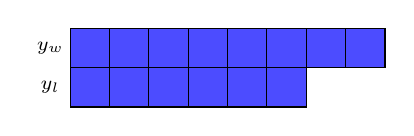
\begin{tikzpicture}[scale=0.5]
                % \node [anchor=north, font=\tiny, align=center]
                % (eq01) at (0,0) {$\beta r(y^w,\pi_{ref})-\beta r(y^l,\pi_{ref})$}
                \foreach \i in {1,...,8} {
                    \draw[fill=blue!70] (\i, 1) rectangle (\i+1, 2);
                }
                \foreach \i in {1,...,6} {
                    \draw[fill=blue!70] (\i, 0) rectangle (\i+1, 1);
                }
                \node at (0.5, 1.5) {\scriptsize $y_w$};
                \node at (0.5, 0.5) {\scriptsize $y_l$};
                % \node at (0.0, 2.5) {\scriptsize $\beta r(y^w,\pi_{ref})-\beta r(y^l,\pi_{ref})$};
            \end{tikzpicture}
        }
        \hspace{0.15in}
        \subfloat[SimPO]{
            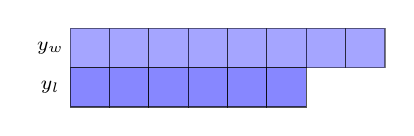
\begin{tikzpicture}[scale=0.5]
                \foreach \i in {1,...,8} {
                    \draw[fill=blue!70,opacity=0.5] (\i, 1) rectangle (\i+1, 2);
                }
                \foreach \i in {1,..., 6} {
                    \draw[fill=blue!70,opacity=0.67] (\i, 0) rectangle (\i+1, 1);
                }
                \node at (0.5, 1.5) {\scriptsize $y_w$};
                \node at (0.5, 0.5) {\scriptsize $y_l$};
                % \node at (0.0, 2.5) {\scriptsize $\beta r(y^w,\pi_{ref})-\beta r(y^l,\pi_{ref})$};
            \end{tikzpicture}
        }
        \hspace{0.15in}
        \subfloat[SamPO]{
            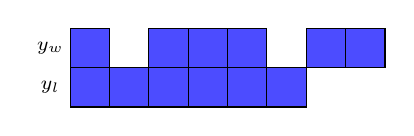
\begin{tikzpicture}[scale=0.5]
                \foreach \i in {1,3,4,5,7,8} {
                    \draw[fill=blue!70] (\i, 1) rectangle (\i+1, 2);
                }
                \foreach \i in {1,...,6} {
                    \draw[fill=blue!70] (\i, 0) rectangle (\i+1, 1);
                }
                \foreach \i in {2, 6} {
                    \draw[fill=blue!70,opacity=0] (\i, 1) rectangle (\i+1, 2);
                }
                \node at (0.5, 1.5) {\scriptsize $y_w$};
                \node at (0.5, 0.5) {\scriptsize $y_l$};
            \end{tikzpicture}
        }
        \hspace{0.15in}
        \subfloat[\method (Ours)]{
            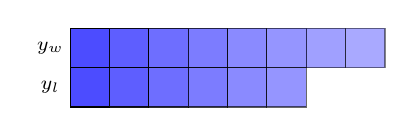
\begin{tikzpicture}[scale=0.5]
                \foreach \i in {1,...,8} {
                    \pgfmathsetmacro{\opacity}{0.9^(\i - 1)};
                    \draw[fill=blue!70,opacity=\opacity] (\i, 1) rectangle (\i+1, 2);
                }
                \foreach \i in {1,...,6} {
                    \pgfmathsetmacro{\opacity}{0.9^(\i - 1)};
                    \draw[fill=blue!70,opacity=\opacity] (\i, 0) rectangle (\i+1, 1);
                }
                \node at (0.5, 1.5) {\scriptsize $y_w$};
                \node at (0.5, 0.5) {\scriptsize $y_l$};
            \end{tikzpicture}
        }
    \end{minipage}
    \begin{minipage}{0.1\textwidth}
        \centering
        \begin{tikzpicture}
            \begin{axis}[
                hide axis,
                scale only axis,
                height=2.8cm,
                width=0.6cm,
                colorbar,
                colormap name=custom_blue, % 你可以选择其他的色彩图,例如 'hot', 'cool', 'jet', 'parula' 等
                point meta min=0,
                point meta max=1,
                colorbar style={
                    ytick={0, 0.2, 0.4,..., 1.0},
                    % ylabel={\scriptsize Weight},
                    yticklabel style={font=\tiny,
                    /pgf/number format/fixed,/pgf/number format/fixed zerofill,/pgf/number format/precision=1},
                },
            ]
            \addplot [draw=none] coordinates {(0,0) (1,1)};
            \end{axis}
        \end{tikzpicture}
        
    \end{minipage}

    \caption{Illustration of coefficients in DPO, SimPO, SamPO, and our \method across various positions. Each box represents a coefficient, and the opacity denotes the magnitude, with darker colors indicating higher values. (a) For DPO, the coefficients are uniform across different positions. (b) For SimPO, the coefficients of the chosen $y_w$ and the rejected $y_l$ are normlaized by their lengths $|y_w|$ and $|y_l|$, respectively. (c) In SamPO, the coefficients are selected based on the minimum length of $|y_w|$ and $|y_l|$. (d) Our method introduces a $\gamma$ factor to implement coefficient decay, specifically as a sequence defined by $\gamma^t$ (e.g., 1, $\gamma$, $\gamma^2$, ..., $\gamma^T$). Here, we use $\gamma=0.9$ for a clear visualization.}
    \label{fig:decay_mechanisms}
\end{figure}



% \newlength{\seg}
%     \setlength{\seg}{2.0em}
%     \newlength{\subseg}
%     \setlength{\subseg}{8em}
%     \newlength{\resseg}
%     \setlength{\resseg}{1.3em}

% \begin{figure}[t]
%     \centering
%     \begin{minipage}{0.78\textwidth}
%         \centering

%         \tikzstyle{rectanglenode}=[rectangle,minimum height=1.5em,minimum width=1.5em, inner sep=0,fill=blue!70, draw=black, line width=0pt];
        
%         \subfloat[DPO]{
%             \begin{tikzpicture}[scale=0.5]
%                 \node [anchor=north, font=\tiny, align=center]
%                 (eq01) at (0,0) {$\beta r(y^w,\pi_{ref})-\beta r(y^l,\pi_{ref})$ };

                
%                 \foreach \i in {1,...,8} {
%                     \node[rectanglenode] at (\i+0.5, 1.5) {};
%                 }
%                 \foreach \i in {1,...,6} {
%                     \node[rectanglenode] at (\i+0.5, 0.5) {};
%                 }
%                 \node at (0.5, 1.5) {\scriptsize $y_w$};
%                 \node at (0.5, 0.5) {\scriptsize $y_l$};
%             \end{tikzpicture}
%         }
        % \hspace{0.15in}
        % \subfloat[SimPO]{
        %     \begin{tikzpicture}[scale=0.5]
        %         \foreach \i in {1,...,8} {
        %             \draw[fill=blue!70,opacity=0.5] (\i, 1) rectangle (\i+1, 2);
        %         }
        %         \foreach \i in {1,..., 6} {
        %             \draw[fill=blue!70,opacity=0.67] (\i, 0) rectangle (\i+1, 1);
        %         }
        %         \node at (0.5, 1.5) {\scriptsize $y_w$};
        %         \node at (0.5, 0.5) {\scriptsize $y_l$};
        %         % \node at (0.0, 2.5) {\scriptsize $\beta r(y^w,\pi_{ref})-\beta r(y^l,\pi_{ref})$};
        %     \end{tikzpicture}
        % }
        % \hspace{0.15in}
        % \subfloat[SamPO]{
        %     \begin{tikzpicture}[scale=0.5]
        %         \foreach \i in {1,3,4,5,7,8} {
        %             \draw[fill=blue!70] (\i, 1) rectangle (\i+1, 2);
        %         }
        %         \foreach \i in {1,...,6} {
        %             \draw[fill=blue!70] (\i, 0) rectangle (\i+1, 1);
        %         }
        %         \foreach \i in {2, 6} {
        %             \draw[fill=blue!70,opacity=0] (\i, 1) rectangle (\i+1, 2);
        %         }
        %         \node at (0.5, 1.5) {\scriptsize $y_w$};
        %         \node at (0.5, 0.5) {\scriptsize $y_l$};
        %     \end{tikzpicture}
        % }
        % \hspace{0.15in}
        % \subfloat[Ours]{
        %     \begin{tikzpicture}[scale=0.5]
        %         \foreach \i in {1,...,8} {
        %             \pgfmathsetmacro{\opacity}{0.9^(\i - 1)};
        %             \draw[fill=blue!70,opacity=\opacity] (\i, 1) rectangle (\i+1, 2);
        %         }
        %         \foreach \i in {1,...,6} {
        %             \pgfmathsetmacro{\opacity}{0.9^(\i - 1)};
        %             \draw[fill=blue!70,opacity=\opacity] (\i, 0) rectangle (\i+1, 1);
        %         }
        %         \node at (0.5, 1.5) {\scriptsize $y_w$};
        %         \node at (0.5, 0.5) {\scriptsize $y_l$};
        %     \end{tikzpicture}
        % }
%     \end{minipage}
%     \begin{minipage}{0.1\textwidth}
%         \centering
%         \begin{tikzpicture}
%             \begin{axis}[
%                 hide axis,
%                 scale only axis,
%                 height=2.8cm,
%                 width=0.6cm,
%                 colorbar,
%                 colormap name=custom_blue, % 你可以选择其他的色彩图,例如 'hot', 'cool', 'jet', 'parula' 等
%                 point meta min=0,
%                 point meta max=1,
%                 colorbar style={
%                     ytick={0, 0.2, 0.4,..., 1.0},
%                     % ylabel={\scriptsize Weight},
%                     yticklabel style={font=\tiny,
%                     /pgf/number format/fixed,/pgf/number format/fixed zerofill,/pgf/number format/precision=1},
%                 },
%             ]
%             \addplot [draw=none] coordinates {(0,0) (1,1)};
%             \end{axis}
%         \end{tikzpicture}
%     \end{minipage}

%     \caption{Illustration of coefficients in DPO, SimPO, SamPO, and our method, across various positions. Each box represents a coefficient, and the opacity denotes the dark color denotes a higher. (a) For DPO, the coefficients are uniform across different positions. (b) For SimPO, the coefficients of the chosen $y_w$ and the rejected $y_l$ are normlaized by its length $|y_w|$ and $|y_l|$, respectively. (c) In SamPO, the coefficients are selected based on the minimum length of $|y_w|$ and $|y_l|$. (d) Our method introduces a $\gamma$ factor controlling the coefficients, which decay according to $\gamma^t$ (e.g., 1, $\gamma$, $\gamma^2$, ..., $\gamma^T$).}
%     \label{fig:decay_mechanisms}
% \end{figure}






\subsection{Temporal decay matters in preference learning.} 

\begin{wrapfigure}[12]{r}{5.1cm}
    \centering
    \vspace{-1.2em}
    \begin{tikzpicture}
    \scriptsize{
    \begin{axis}[
        width=.38\textwidth, height=.32\textwidth,
        xlabel=Response Position,
        ylabel=Probability,
        xmin=0, xmax=1050,
        ymin=0.73, ymax=1.01,
        xtick={0,200,400,600,800,1000, 1200,1400},
        % xticklabels={$0$,$10$,$20$,$30$,$40$,$50$},
        ytick={0.70, 0.80, 0.90, 1.0},
        % yticklabels={$0.1$,$0.2$,$0.3$,$0.4$,$0.5$,$0.6$},
        ymajorgrids=true,
        xmajorgrids=true,
        grid style=dashdotted,
        legend cell align=left,
        scaled ticks=false,
        xlabel style={align=center,font=\scriptsize},
        ylabel style={font=\scriptsize,yshift=0em},
        yticklabel style={
            /pgf/number format/fixed,
            /pgf/number format/fixed zerofill,
            /pgf/number format/precision=1
        },
        ytick style={opacity=0},
        % xtick label style={font=\tiny},
        % ytick label style={font=\tiny},
        legend style={
            yshift=-0.2em,
            xshift=-2.9em,
            legend cell align=left,
            legend plot pos=right,
            fill opacity=0.5, draw opacity=0.5
        },
    ]
    \addplot [
        only marks,
        red,
        mark size=0.3pt,
        thick,] table [
        x=position,
        y=value,
        col sep=comma
    ] {./Figure/llama_chosen_prob_distribution.csv};

    \addplot [
        only marks,
        blue,
        mark size=0.3pt,
        thick,] table [
        x=position,
        y=value,
        col sep=comma
    ] {./Figure/gemma_chosen_prob_distribution.csv};

    \addplot [
        only marks,
        teal,
        mark size=0.3pt,
        thick,] table [
        x=position,
        y=value,
        col sep=comma
    ] {./Figure/mistral_chosen_prob_distribution.csv};
    \legend{\tiny{Llama3-Instruct (8B)},\tiny{Gemma2-Instruct (9B)},\tiny{Mistral-NeMo-Instruct (12B)}},
    \end{axis}}
    \end{tikzpicture}
    \vspace{-0.7em}
    \caption{Probability against positions on 1000 samples.}
     \label{fig:pred_prob}
\end{wrapfigure}


% \begin{wrapfigure}[13]{r}{5.1cm}
    % \centering
    % \vspace{-1.2em}
    % \begin{tikzpicture}
    %   \scriptsize{
    %   \begin{axis}[
    %   width=.38\textwidth, height=.32\textwidth ,
    %   xlabel=Response Position,
    %   ylabel=Probability,
    %   xmin=0, xmax=1050,
    %   ymin=0.7, ymax=1.01,
    %   xtick={0,200,400,600,800,1000, 1200,1400},
    %   %xticklabels={$0$,$10$,$20$,$30$,$40$,$50$},
    %   ytick={0.70, 0.80..., 1.0},
    %   % yticklabels={$0.1$,$0.2$,$0.3$,$0.4$,$0.5$,$0.6$},
    %   ymajorgrids=true,
    %   xmajorgrids=true,
    %   grid style=dashdotted,
    %   legend cell align=left,
    %   scaled ticks=false,
    %   xlabel style={align=center,font=\scriptsize},
    %   ylabel style={font=\scriptsize,yshift=0em},
    %   yticklabel style={/pgf/number format/fixed,/pgf/number format/fixed zerofill,/pgf/number format/precision=1},
    %   ytick style={opacity=0},
    %   % xtick label style={font=\tiny},
    %   % ytick label style={font=\tiny},
    %   legend style={yshift=-7.2em,xshift=0em,legend cell align=left,legend plot pos=right},
    %   ]
    %   \addplot [only marks,blue,mark size=3pt,thick,line width=0.5pt,mark size=0.2pt] table [x=position,y=value,col sep=comma] {./Figure/gemllama_chosen_prob_distribution.csv}};
    %   % \legend{\tiny{Llama3-Instruct (8B)}},
    %   \end{axis}}

      
    %   }
    %   \end{tikzpicture}
    % \caption{Visualization of }
    %  \label{fig:pred_prob}
    % \end{wrapfigure}

\paragraph{Motivation.}
Preference learning plays a pivotal role in optimizing LLMs, especially when leveraging user feedback to align model outputs with human preferences. While methods like DPO~\citep{Rafailov2023DirectPO} and its successors~\citep{Meng2024SimPO,lu2024sampo} have demonstrated significant potential in this domain, they exhibit a critical oversight: the uniform treatment of tokens across the sequence. As illustrated in Figure \ref{fig:decay_mechanisms}, DPO, SimPO, and SamPO assign identical coefficients to all tokens within the chosen response $y_w$ and the rejected response $y_l$. We argue that optimizing each token equally, without considering their positional importance or temporal dependence, is suboptimal for most scenarios.

Our observations indicate that earlier tokens receive greater optimization during the preference learning process compared to later ones (see Figure \ref{fig:self_sampling}
). This suggests that the benefits derived from the alignment phase over SFT are predominantly due to the optimization of initial tokens. Additionally, when plotting the prediction probability across different response positions in Figure \ref{fig:pred_prob}, we find that more recent tokens have higher probabilities than earlier tokens. This indicates that the model becomes increasingly confident in predicting tokens as it progresses through the sequence, likely due to the accumulating contextual information from previous tokens. However, since the accuracy of these later tokens is already high—reaching up to 0.9, further improvements are more likely to come from enhancing the accuracy of the earlier tokens. Therefore, a natural approach is to focus on improving the accuracy of the prefix: \textit{the more accurate the earlier tokens are, the better the overall quality of the sequence will be.}

\vspace{-0.25cm}
\paragraph{Temporal Decay Mechanism.} Inspired by the success of \citet{yang2024denseReward}, where earlier steps are crucial in the reverse chain of the diffusion denoising process, we propose a temporal decay mechanism to highlight the importance of earlier tokens in LLM scenarios. Considering the original DPO loss formulation, the most direct way to prioritize earlier tokens is to incorporate a position-dependent coefficient that decays over time. Multiple decay mechanisms can achieve this, including linear, polynomial, step, and cosine decay functions. After evaluating these options, we chose exponential decay due to its simplicity and effectiveness.

Exponential decay applies a coefficient that decreases exponentially with the token position, represented as $\gamma^t$, where $\gamma$ is the decay rate ($0 < \gamma < 1$) and $t$ is the token's position. This approach provides a smooth and gradual reduction in the influence of later tokens, ensuring that earlier tokens have a more significant impact on the loss calculation. To this end, we adapt this concept to the DPO loss function which defined as:
% Drawing inspiration from reinforcement learning, where rewards are discounted over time using an exponential function to model time preference, 
\sethlcolor{red}
\begin{equation}
\label{eq:d^2po}
\mathcal{L}_{\textrm{D}^2\textrm{PO}}\left(\pi_\theta ; \pi_{\mathrm{ref}}\right)
    =-\log \sigma\left(\sum\limits_{t=0}^{T_w} \textcolor{red}{\gamma^t} \beta \log \frac{\pi_\theta\left(\mathbf{y}_w^t \mid \mathbf{x},\mathbf{y}_w^{<t}\right)}{\pi_{\mathrm{ref}}\left(\mathbf{y}_w^t \mid \mathbf{x},\mathbf{y}_w^{<t}\right)}-\sum\limits_{t=0}^{T_l} \textcolor{red}{\gamma^t} \beta \log \frac{\pi_\theta\left(\mathbf{y}_l^t \mid \mathbf{x},\mathbf{y}_l^{<t}\right)}{\pi_{\mathrm{ref}}\left(\mathbf{y}_l^t \mid \mathbf{x},\mathbf{y}_l^{<t}\right)}\right)
\end{equation}
\noindent In this formulation, the exponential decay factor $\gamma^t$ adjusts the contribution of each token based on its position in the sequence. As is shown in Figure \ref{fig:decay_mechanisms} (d), coefficients of each token in \method gradually decrease along the position (the color from dark to light), placing greater emphasis on earlier tokens. This modification aligns the optimization process with the observed pattern of optimization in preference learning, where initial tokens benefit more from the alignment phase. Similar to the derivation of the vanilla DPO, we provide the detailed derivation of \method in the Appendix \ref{sec:derivation}.

    
\subsection{Reference-free is consistent with on-policy setups.} 
\label{sec:reference-free}

\begin{wrapfigure}[9]{r}{5.4cm}
    \centering
    \vspace{-0.5cm}
    \begin{tikzpicture}
    \scriptsize{
        \begin{axis}[
            width=5.0cm,
            height=3.6cm,
            xlabel={Ref margin. $\pi_{\text{ref}} (y_w|x) - \pi_{\text{ref}} (y_l|x)$},
            ylabel={Density},
            xmin=-100, xmax=100,
            ymin=0, ymax=0.12,
            legend style={at={(0.73, 1.0)}, anchor=north, legend columns=1, fill opacity=0.5, draw opacity=0.5},
            % axis lines=left,
            % grid=major,
            ymajorgrids=true,
            xmajorgrids=true,
            grid style=dashdotted,
            legend cell align=left,
            scaled ticks=false,
            ytick={0.02, 0.04,..., 0.12},
            xtick={-100,-50,0,50,100},
            yticklabel style={/pgf/number format/fixed,/pgf/number format/fixed zerofill,/pgf/number format/precision=2, rotate=0},
            enlargelimits=false,
            domain=-100:100,
            samples=200,
        ]
        % Plot 1: Self Sampling (blue curve)
        \addplot [
            thick,
            blue,
            fill=blue,
            fill opacity=0.2
        ]
        table[x=value, y=density, col sep=comma] {Figure/llama_self_sampling_ref_margin.csv} \closedcycle;

        \addlegendentry{\tiny{On-Policy}}
        % Plot 2: Non Self Sampling (orange curve)
        \addplot [
            thick,
            orange,
            fill=orange,
            fill opacity=0.2
        ]
        table[x=value, y=density, col sep=comma] {Figure/llama_non_self_sampling_ref_margin.csv} \closedcycle;
        \addlegendentry{\tiny{Off-Policy}}
        
        % Vertical dashed line at x = 0
        % \addplot[dashed, thick, blue] coordinates {(4, 0) (4, 0.76)};
        
        \end{axis}}
    \end{tikzpicture}
    \vspace{-0.45em}
    \caption{Reference margin of DPO.}
    \label{fig:ref_margin_density}
\end{wrapfigure}
Reference-based methods often incorporate a KL divergence constraint to prevent the policy model from deviating significantly from its initial state, which adds computational and memory overhead. In the context of DPO, this constraint appears as an adaptive margin term $\log \frac{\pi_{\text{ref}}(y_l|x)}{\pi_{\text{ref}}(y_w|x)}$ in the pairwise loss function. This term quantifies the reference model's preference difference between less-preferred ($y_l$) and preferred ($y_w$) responses. 
We note that the DPO loss can be viewed as a specific case of contrastive loss, where $\log \pi_\theta(y)$ measures the relevance between the prompt $x$ and the response $y$. The adaptive margin ensures that loss values remain moderate, contributing to training stability. However, if the reference model assigns similar probabilities to both $y_w$ and $y_l$ (i.e., the margin approaches zero), the impact of the reference model diminishes, suggesting that it can be easily excluded.


To validate this, we analyze the margin distributions in the UltraFeedback dataset under off-policy and on-policy settings. In the off-policy setting, we use original responses, while in the on-policy setting, responses are regenerated by the same model. As illustrated in Figure~\ref{fig:ref_margin_density}, the on-policy dataset exhibits smaller variance in margins and an average closer to zero compared to the off-policy dataset. This indicates a higher proportion of semi-hard samples in the on-policy data. From this perspective, we can discard the KL divergence constraint under on-policy settings and easily derive the reference-free version loss function:
\begin{equation}
\mathcal{L}_{\textrm{D}^2\textrm{PO}}\left(\pi_\theta\right)
    =-\log \sigma\left(\sum\limits_{t=0}^{T_w} \gamma^t \beta \log \pi_\theta\left(\mathbf{y}_w^t \mid \mathbf{x,y_w^{<t}}\right)-\sum\limits_{t=0}^{T_l} \gamma^t \beta \log \pi_\theta\left(\mathbf{y}_l^t \mid \mathbf{x,y_l^{<t}}\right)\right)
\end{equation}
\section{theoretical analysis}
In this section, we analyze the influence of the discount factor $\gamma$ on the performance of our method compared to DPO. Both DPO and our method can be considered as a token-level MDP that satisfies the Bellman equation. Here, we define the suboptimality as the performance difference between the optimal policy $\pi^{*}$ and a given policy $\pi$ under specific discount factors, which has been widely discussed in offline RL~\citep{rashidinejad2021bridging,jin2021pessimism}.

\subsection{Suboptimality Decomposition}
\textbf{Definition 1 (Suboptimality).} The suboptimality of a policy $\pi$ with respect to the optimal policy $\pi^*$, starting from an initial state $s$ under discount factor $\gamma$, is defined as:
\begin{equation}
\text{SubOpt}(\pi, s; \gamma) = V_{\gamma}^{\pi^*}(s) - V_{\gamma}^{\pi}(s),
\end{equation}
where $V_{\gamma}^{\pi}(s) = \mathbb{E}_{\pi}\left[\sum_{t=0}^{H-1} \gamma^{t} r(s_t, a_t) \mid s_0 = s\right]$ is the expected return of policy $\pi$ under discount factor $\gamma$, and $H$ is the finite horizon. To analyze the influence of the discount factor $\gamma$, we consider the suboptimality of our method evaluated with an evaluation discount factor $\gamma_e = 1.0$. We decompose the suboptimality into three terms that separately capture the differences due to the discount factors and the policy discrepancies. In this way, we can rewrite the suboptimality as below:
\begin{equation}
\begin{aligned}
\text{SubOpt}(\pi, s; \gamma_e) &= V_{\gamma_e}^{\pi^*}(s) - V_{\gamma_e}^{\pi}(s) \\
&= \underbrace{\left[V_{\gamma_e}^{\pi^*}(s) - V_{\gamma}^{\pi^*}(s)\right]}_{\Delta_1} + \underbrace{\left[V_{\gamma}^{\pi^*}(s) - V_{\gamma}^{\pi}(s)\right]}_{\Delta_2} + \underbrace{\left[V_{\gamma}^{\pi}(s) - V_{\gamma_e}^{\pi}(s)\right]}_{\Delta_3}
\end{aligned}
\end{equation}

This decomposition allows us to separately analyze the impact of the discount factors and the policy differences.

\subsection{Suboptimality Analysis}
\textbf{Theorem 1(Suboptimality Upper Bound).} 
\emph{Let $\pi^*$ denote the optimal policy, and $\pi$ be the policy under a discount factor $\gamma \in [0, 1)$. Assume that rewards are bounded such that $\left| r(s, a) \right| \leq R$ for all states $s$ and actions $a$, and consider a finite horizon $H$. Then, the suboptimality of $\pi$ compared to $\pi^*$ when evaluated with an evaluation discount factor $\gamma_e = 1.0$ satisfies the following upper bound:}
\begin{equation}
\begin{aligned}
\text{SubOpt}(\pi,s; \gamma_e) \leq 2(H - \frac{1-\gamma^H}{1-\gamma})R + \frac{2(1-\gamma^H)^2}{(1-\gamma)^2}E_{s \sim d^{\pi^{*}}}\left[\mathbb{TV}(\pi^*(a|s)||\pi(a|s)\right]R
\end{aligned}
\end{equation}

The complete proof is included in Appendix \ref{sec:theorem_proof}. This upper bound reveals that the suboptimality depends on both the discount factor $\gamma$ and the mismatch between $\pi$ and $\pi^*$. Specifically, the first term $H - \frac{1 - \gamma^{H}}{1 - \gamma}$ decreases as $\gamma$ increases, while the second term $\left(\frac{1 - \gamma^{H}}{1 - \gamma}\right)^2$ increases, highlighting a trade-off in the choice of $\gamma$. As both terms vary monotonically with the discount factor $\gamma$ but in opposing directions, there exists an optimal value $\gamma^*$ within the interval $(0, 1)$ that balances these effects to minimize the overall suboptimality.

\section{Experiments}

\subsection{Experimental Setups}
\label{sec:baselines}
Due to page limitations, we briefly describe the model setting, training data, and hyperparameters in the following section. Expanded details on evaluation benchmarks and baselines are available in Appendix \ref{appendix:exp_setup}.
\paragraph{Model Setting.} We conducted preference optimization experiments using three model families: Llama3-8B~\citep{llama3modelcard}, Gemma2-9B~\citep{gemmateam2024gemma2improvingopen} and Mistral-12B~\citep{Jiang2023Mistral7}. Here, we mainly focused on building our systems upon the instruct models.
Thus, we utilized pre-trained instruction-tuned models (e.g., \href{https://huggingface.co/meta-llama/Meta-Llama-3-8B-Instruct}{meta-llama/Meta-Llama-3-8B-Instruct}, \href{https://huggingface.co/google/gemma-2-9b-it}{google/gemma-2-9b-it}, and \href{https://huggingface.co/nvidia/Mistral-NeMo-12B-Instruct}{nvidia/Mistral-NeMo-12B-Instruct}) as the SFT models.\footnote{The exact nature of the instruction-tuning (whether it includes SFT or the complete RLHF pipeline) of these models is not fully disclosed. For simplicity, we refer to these as SFT models.} 

\vspace{-0.25cm}
\paragraph{Training Data}
Our experiments were carried out using the UltraFeedback dataset. Specifically, We categorize the preference data into two types: 1) off-policy data (original response pairs from the UltraFeedback dataset), and 2) on-policy data generated using the SFT models. Similar to SimPO~\citep{Meng2024SimPO}, for each prompt $x$, we generated 5 responses using the SFT model with a sampling temperature of 0.8. To validate these responses, we employed \href{https://huggingface.co/RLHFlow/ArmoRM-Llama3-8B-v0.1}{{RLHFlow/ArmoRM-Llama3-8B-v0.1}}~\citep{ArmoRM} to assign scores to each response, allowing us to select the highest-scoring response as $y_w$ and the lowest-scoring one as $y_l$.

\vspace{-0.25cm}
\paragraph{Hyperparameters}
For all models, we set the maximum response length to 2,048 tokens and used a batch size of 128. Optimization was performed using the AdamW optimizer~\citep{kingma2014adam} with a learning rate of $5e-7$ and a cosine learning rate schedule featuring a 10\% warmup period. In preference optimization methods, including DPO and its variants such as our method \method{} and SamPO, we set $\beta$ to 0.1 to ensure a fair comparison.


\begin{table*}[!t]
\setlength{\tabcolsep}{2pt}
\centering
\small 
\caption{We report AlpacaEval 2~\citep{AlpacaEval} (denoted by AE2), Arena-Hard~\citep{arenahard2024} (denoted by AH), and MT-Bench~\citep{zheng2023judging} (denoted by MB) results under three settings using standard provided samples. Note that LC and WR denote length-controlled and raw win rate, respectively. We used off-the-shelf models as the SFT model. And our judge model is GPT-4-Turbo.}

% \resizebox{\textwidth}{!}{
\begin{tabular}{lcccccccccccc}
% \begin{tabular}{lrrrrrrrrrr}
\toprule
\multirow{3}{*}{\textbf{Method}} & \multicolumn{4}{c}{\textbf{Llama3-Instruct (8B)}} & \multicolumn{4}{c}{\textbf{Gemma2-Instruct (9B)}} & \multicolumn{4}{c}{\textbf{Mistral-NeMo-Instruct (12B)}} \\ 
\cmidrule(lr){2-5}\cmidrule(lr){6-9}\cmidrule(lr){10-13}
& \multicolumn{2}{c}{\textbf{AE2}} & \multicolumn{1}{c}{\textbf{AH}} & \multicolumn{1}{c}{\textbf{MB}} & \multicolumn{2}{c}{\textbf{AE2}} & \multicolumn{1}{c}{\textbf{AH}} & \multicolumn{1}{c}{\textbf{MB}} & \multicolumn{2}{c}{\textbf{AE2}} & \multicolumn{1}{c}{\textbf{AH}} & \multicolumn{1}{c}{\textbf{MB}} \\
\cmidrule(lr){2-3}\cmidrule(lr){4-4} \cmidrule(lr){5-5} \cmidrule(lr){6-7}\cmidrule(lr){8-8}\cmidrule(lr){9-9} \cmidrule(lr){10-11}\cmidrule(lr){12-12}\cmidrule(lr){13-13} 
& {\scriptsize \bf WR (\%)} & {\scriptsize \bf LC (\%)} & {\scriptsize \bf WR (\%)} & {\scriptsize \bf G4-T} & {\scriptsize \bf WR (\%)}  & {\scriptsize \bf LC (\%)} & {\scriptsize \bf WR (\%)} & {\scriptsize \bf G4-T} & {\scriptsize \bf WR (\%)}  & {\scriptsize \bf LC (\%)} & {\scriptsize \bf WR (\%)} & {\scriptsize \bf G4-T} \\
\midrule
SFT          & 39.1  & 40.1  & 27.6  & 7.5 & 37.6 & 47.2 & 44.1 & 8.3 & 44.6 & 47.7 & 46.5 & 8.1 \\
\midrule
DPO          & 37.4 & 40.3 & 27.7 & \textbf{7.7} & 38.8 & 48.8 & 42.5 & 8.1 & 44.4 & 49.3 & 48.5 & 8.3 \\
KTO          & 33.3 & 38.1 & 21.0 & 7.5 & 39.1 & 50.0 & 43.8 & 8.3 & 37.4 & 48.7 & 35.8 & 8.2 \\
IPO          & 42.2 & \textbf{45.7} & 31.9 & 7.6 & 41.0 & 50.0 & 48.2 & 8.0 & 39.8 & 48.9 & 39.8 & 8.2 \\
SamPO          & 40.7 & 43.1 & 26.1 & 7.5 & 39.9 & 50.1 & 46.9 & 8.2 & 43.5 & 49.5 & 50.1 & 8.1 \\
$\textrm{D}^2$PO (ours) & \textbf{43.5} & 43.0 & \textbf{37.0} & \textbf{7.7} & \textbf{45.5} & \textbf{51.0} & \textbf{50.2} & \textbf{8.3} & \textbf{51.3} & \textbf{54.4} & \textbf{51.8} & \textbf{8.4} \\
\midrule
ORPO         & 10.6 & 15.3 & 6.8 & 6.3 & 11.3 & 21.6 & 10.2 & 7.1 & 9.6 & 17.0 & 9.8 & 6.9 \\
SimPO        & 0.3$^*$ & 0.8$^*$ & 1.4$^*$ & 1.6$^*$ & 38.8 & 50.0 & 31.6 & 8.0 & 46.8 & \textbf{53.3} & 46.6 & 8.0 \\
\bottomrule
\end{tabular}
% }
\label{tab:main_res_offline_turbo}
\vspace{-.5em}
\end{table*}


\begin{table*}[!t]
\setlength{\tabcolsep}{2pt}
\centering
\small 
\caption{Following the setting in \citet{Meng2024SimPO}, we used the on-policy data to obtain the chosen and rejected and applied a stronger reward model. $\dagger$ denotes our reference-free version.}
% \resizebox{\textwidth}{!}{
\begin{tabular}{lcccccccccccc}
% \begin{tabular}{lrrrrrrrrrr}
\toprule
\multirow{3}{*}{\textbf{Method}} & \multicolumn{4}{c}{\textbf{Llama3-Instruct (8B)}} & \multicolumn{4}{c}{\textbf{Gemma2-Instruct (9B)}} & \multicolumn{4}{c}{\textbf{Mistral-NeMo-Instruct (12B)}} \\ 
\cmidrule(lr){2-5}\cmidrule(lr){6-9}\cmidrule(lr){10-13}
& \multicolumn{2}{c}{\textbf{AE2}} & \multicolumn{1}{c}{\textbf{AH}} & \multicolumn{1}{c}{\textbf{MB}} & \multicolumn{2}{c}{\textbf{AE2}} & \multicolumn{1}{c}{\textbf{AH}} & \multicolumn{1}{c}{\textbf{MB}} & \multicolumn{2}{c}{\textbf{AE2}} & \multicolumn{1}{c}{\textbf{AH}} & \multicolumn{1}{c}{\textbf{MB}} \\
\cmidrule(lr){2-3}\cmidrule(lr){4-4} \cmidrule(lr){5-5} \cmidrule(lr){6-7}\cmidrule(lr){8-8}\cmidrule(lr){9-9} \cmidrule(lr){10-11}\cmidrule(lr){12-12}\cmidrule(lr){13-13} 
& {\scriptsize \bf WR (\%)} & {\scriptsize \bf LC (\%)} & {\scriptsize \bf WR (\%)} & {\scriptsize \bf G4-T} & {\scriptsize \bf WR (\%)}  & {\scriptsize \bf LC (\%)} & {\scriptsize \bf WR (\%)} & {\scriptsize \bf G4-T} & {\scriptsize \bf WR (\%)}  & {\scriptsize \bf LC (\%)} & {\scriptsize \bf WR (\%)} & {\scriptsize \bf G4-T} \\
\midrule
SFT          & 39.1 & 40.1 & 27.6 & 7.5 & 37.6 & 47.2 & 44.1 & 8.3 & 44.6 & 47.7 & 46.5 & 8.1 \\
\midrule
DPO          & 46.2 & 47.6 & 42.4 & 7.8 & 47.0 & 53.4 & 56.7 & \textbf{8.4} & 53.5 & 53.3 & 59.0 & 8.4 \\
KTO          & 42.4 & 44.8 & 32.1 & 7.7 & 48.3 & 53.4 & 57.1 & 8.3 & 48.9 & 51.9 & 53.2 & 8.4 \\
IPO          & 42.9 & 46.0 & 34.5 & 7.9 & 50.9 & 50.0 & 59.7 & 8.3 & 53.6 & 54.4 & 59.7 & 8.4 \\
SamPO        & 44.4 & 47.2 & 35.8 & \textbf{8.0} & 45.8 & 55.2 & 55.2 & 8.2 & 51.1 & 53.0 & 58.3 & 8.3 \\
$\textrm{D}^2$PO (ours) & \textbf{47.4} & \textbf{53.5} & \textbf{47.3} & 7.8 & \textbf{57.2} & \textbf{59.7} & \textbf{66.4} & 8.3 & \textbf{57.3} & \textbf{62.1} & \textbf{62.3} & \textbf{8.6} \\
\midrule
ORPO         & 37.8 & 39.3 & 25.5 & 7.7 & 41.9 & 51.1 & 45.3 & 8.2 & 43.8 & 47.5 & 46.0 & 8.2 \\
SimPO        & 44.4 & 50.3 & 41.9 & \textbf{7.8} & 54.5 & 58.4 & 65.0 & \textbf{8.3} & 51.3 & 55.0 & 61.9 & \textbf{8.3} \\
$\textrm{D}^2$PO$^\dagger$ (ours)    & \textbf{48.0} & \textbf{53.9} & \textbf{46.1} & 7.7 & \textbf{56.7} & \textbf{60.8} & \textbf{65.7} & \textbf{8.3} & \textbf{58.3} & \textbf{62.4} & \textbf{63.6} & \textbf{8.3}\\
\bottomrule
\end{tabular}
% }
\label{tab:main_res_online_turbo}
\vspace{-.5em}
\end{table*}

\subsection{Experimental Results}
In our experiments, we provide a comprehensive comparison of our proposed method against DPO and its variants on both off-policy and on-policy data respectively, along with the baselines introduced in Section \ref{sec:baselines}. The baselines are categorized into two broad paradigms: reference-based and reference-free (SimPO and ORPO). Notably, as discussed in Section \ref{sec:reference-free}, our method can be seamlessly integrated into the reference-free paradigm using on-policy data.
We ensure fair comparisons by maintaining consistency in the codebase and experimental settings across all methods evaluated.

% ############Figure############

\begin{table}[t!]
    \centering
    \setlength{\tabcolsep}{5pt}
    \caption{\textbf{Effect of different kernel bandwidths.} Scoring performance metrics are retrieved and averaged over 5 independent runs.}
\vspace{3mm}
\resizebox{0.8\linewidth}{!}{
\begin{tabular}{l cc }
\toprule
 \textbf{Kernel Bandwidth} & $\textbf{Spearman} \uparrow$ & $\textbf{Pearson} \uparrow$ \\
 \midrule
    $\gamma = $ Median & 0.999	& 0.993	\\
\midrule
    $\gamma = 0.001$ & 0.999	& 0.994	 \\
    $\gamma = 0.01$ & 0.999	& 0.994	\\
    $\gamma = 0.1$ & 0.999	& 0.994	 \\
    $\gamma = 1.0$ & 0.999	& 0.994	 \\
    $\gamma = 10.0$ &  0.801 & 0.838 \\	
\bottomrule
% \vspace{-4mm}
\end{tabular}
}
\vspace{-4mm}
\label{tab:gamma}
\end{table}

% ############Figure############

\vspace{-0.25cm}
\paragraph{Off-policy Setups.}
Table \ref{tab:main_res_offline_turbo} clearly demonstrates that our method delivers significant improvements in win rates across all configurations. Specifically, when applied to the Llama3, our method outperforms DPO by margins of 6.1\% and 2.9\% in standard and length-controlled evaluation scenarios, respectively. Similarly, for the Mistral-NeMo model, our method surpasses DPO by margins of 6.9\% and 5.1\% in standard and length-controlled scenarios, respectively. We observed that reference-free methods exhibited instability when applied to off-policy data, often leading to a degradation in model performance. This issue is particularly evident with SimPO, where previous work observed similar findings~\citep{lu2024sampo}. This phenomenon highlights the challenges associated with reference-free methods in preference optimization on off-policy data.

\vspace{-0.25cm}
\paragraph{On-policy Setups.}
As shown in Table \ref{tab:main_res_online_turbo}, our proposed method, along with all baselines, achieves better results compared to off-policy settings. Notably, our method consistently demonstrates improvements across different setups. Due to the reward model's length preference when selecting on-policy data, models trained on this data are more prone to verbosity. A critical observation in standard evaluations is the inherent bias favoring models that generate longer responses, which tend to achieve higher win rates. However, our method not only achieves superior win rates but also produces significantly shorter responses, showcasing its efficiency in generating concise and relevant outputs. Additionally, when the reference model is omitted, our method outperforms SimPO by 2.4–7.4 in LC win rate and 0.7–4.2 in win rate on AlpacaEval 2 and Arena-Hard, respectively. These findings further underscore the robustness and effectiveness of our approach. This superiority in both reference-based and reference-free contexts emphasizes the versatility and reliability of our method in preference optimization.

\section{Analyses}

\paragraph{$\gamma$ Plays an Important Role.} 
The temporal decay is one of the main contributions of this work, and we would like to show how the $\gamma$ affects the performance. We conducted ablation studies on three open-source models for robust conclusions. Through results as shown in Figure \ref{fig:gamma_vs_winrate}, we see that nearly all variants with $\gamma$ lower than 1.0 consistently outperform DPO\footnote{DPO is a special case of ours where $\gamma$ equals to 1.0.}. Also, $\gamma=0.98$  achieves the highest performance across three benchmarks for these strong open-source models. This indicates that our method is robust to the choice of $\gamma$, reducing the need for extensive hyperparameter tuning.

\setlength{\tabcolsep}{4pt}
\begin{table*}[!t]
\centering
\small 
\caption{Results on OpenLLM Benchmark, including reasoning and mathematical testsets. Note that Hella. denotes Hellaswag, Truth. denotes TruthfulQA and Wino. denotes Winogrande.}

% \resizebox{\textwidth}{!}{
\begin{tabular}{lccccccccccc}
\toprule
\multirow{2}{*}{\textbf{Method}}  & \textbf{MMLU} & \textbf{GSM8K} & \textbf{Math} & \textbf{IFEval} & \textbf{ARC-C} & \textbf{Hella.} & \textbf{Truth.} & \textbf{Wino.} \\ 
\cmidrule(lr){2-9}
& 0-shot & 0-shot & 0-shot & 0-shot & 25-shot & 10-shot & 0-shot & 5-shot \\ 
\midrule
\multicolumn{9}{c}{\bf (a) Llama3-Instruct (8B)} \\
SFT          & 61.7  & 78.5  & 7.9 & 68.6 & 62.0 & 78.8 & 51.6 & 75.5  \\
\midrule
DPO          & 56.7  & 70.5  & 7.8 & 65.1 & 65.1 & \textbf{79.9} & 56.4 & 74.5  \\
SimPO        & 55.2  & 57.5  & 5.3 & 60.8 & \textbf{67.6} & 78.8 & \textbf{63.8} & 74.3  \\
\method (ours) & \textbf{61.4} & \textbf{72.0} & \textbf{8.5} & \textbf{65.6} & 65.8 & 79.0 & 57.6 & \textbf{75.1} \\
\midrule
\multicolumn{9}{c}{\bf (b) Gemma2-Instruct (9B)} \\
SFT          & 72.8 & 87.4  & 19.4 & 71.9 & 71.8 & 81.7 & 60.2	& 77.9  \\
\midrule
DPO          & 72.2	& 88.5 & 19.4 & 60.1 & 69.9	& 71.5 & 57.7 & 72.7  \\
SimPO        & 72.4 & 88.2 & 19.0 & \textbf{71.5} & 68.3	& 66.5 & 58.9 & 73.7  \\
\method (ours) & \textbf{72.7} & \textbf{88.9} & \textbf{21.2} & 71.2 & \textbf{71.4} & \textbf{81.0} & \textbf{61.3} & \textbf{76.0} \\
\bottomrule
\end{tabular}
% }
\label{tab:openllm_benchmark}
\vspace{-.5em}
\end{table*}

\vspace{-0.25cm}
\paragraph{$\gamma$ Larger than 1 is Harmful.} 
As highlighted in the previous section, we prioritize earlier feedback over more recent feedback, aligning with the next-token prediction paradigm. We conducted an experiment where the decay factor $\gamma$ was set to slightly greater than 1.0 to observe the effects. The results could also be observed in Figure \ref{fig:gamma_vs_winrate}. When $\gamma$ exceeds 1.0, rewards linked to later tokens in the sequence receive larger coefficients than those for earlier tokens. However, this adjustment was detrimental to preference optimization, resulting in performance that lagged behind the standard DPO on both the AlpacaEval 2 and Arena-Hard benchmarks. This finding demonstrates the crucial role of earlier tokens in the alignment process and indicates that overemphasizing later tokens can degrade model performance.

\vspace{-0.25cm}
\paragraph{Evaluations on OpenLLM Benchmark.}

To verify whether the improvements of \method on the aforementioned RLHF benchmarks, such as Alpaca Eval2, Arena Hard, and MT-bench, come at the expense of general language modeling ability, we conducted a comprehensive evaluation of downstream tasks on the Open LLM leaderboard\footnote{Open LLM leaderboard is created by huggingface to provide a standardized evaluation setup for LLMs, which includes several popular benchmarks encompassing a wide range of capabilities across multiple domains.}. Specifically, we employed zero-shot evaluations on MMLU~\citep{hendrycks2021measuring}, GSM8K~\citep{cobbe2021training}, MATH~\citep{hendrycks2021measuring}, IFEval~\citep{zhou2023instruction}, and TruthfulQA~\citep{lin2022truthfulqa}. Additionally, we performed few-shot evaluations on ARC-C~\citep{clark2018think}, Hellaswag~\citep{zellers2019hellaswag}, and Winogrande~\citep{levesque2012winograd} according to the official settings in the Open LLM leaderboard. The results are summarized in Table \ref{tab:openllm_benchmark}, and we observe that:

\begin{itemize}[leftmargin=*]
    \item In the Llama3-8B configuration, our \method method significantly outperforms both DPO and SimPO, particularly on the MMLU and MATH benchmarks. Notably, \method exhibits less performance degradation on GSM8K compared to SimPO, despite both methods effectively controlling output length. \method achieves substantial performance gains on the MATH dataset, surpassing the Instruct model by 0.55 points, while the other two methods show a noticeable decline.
    \item In the Gemma2-9B configuration, we observe a similar pattern, with \method demonstrating a significant performance advantage on the MATH benchmark. These results suggest that \method effectively enhances reasoning and mathematical problem-solving abilities in LLMs across different models. Furthermore, these additional evaluations on specialized datasets confirm that \method maintains its effectiveness across various contexts and task types.
\end{itemize}



\begin{table*}[!t]
\centering
\small 
\caption{Comparison of different decay mechanisms in terms of performance and response length.}
\label{tab:decay_methods}
\begin{tabular}{lcccccccc}
\toprule
\multirow{2}{*}{\textbf{Decay Strategy}} & \multirow{2}{*}{\textbf{Rewards}} & \multicolumn{3}{c}{\textbf{AE2}} & \multicolumn{2}{c}{\textbf{AH}} & \multicolumn{1}{c}{\textbf{MB}} \\
\cmidrule(lr){3-5}\cmidrule(lr){6-7}\cmidrule(lr){8-8}
& & {\scriptsize  \bf WR (\%)} & {\scriptsize \bf LC (\%)} & {\scriptsize \bf Len.} & {\scriptsize \bf WR (\%)} & {\scriptsize \bf Len.} & {\scriptsize \bf G4-T} \\
\midrule
Exponential & $\sum\limits_{t=0}^{T} \gamma^t \beta \log \frac{p_\theta\left(\mathbf{y}_t \mid \mathbf{x,y_{<t}}\right)}{p_{ref}\left(\mathbf{y}_t \mid \mathbf{x,y_{<t}}\right)}$ & 57.2 & 59.7 & 1950 & 66.4 & 724 & 8.3 \\

Head & $\sum\limits_{t=0}^{\gamma T} \beta \log \frac{p_\theta\left(\mathbf{y}_t \mid \mathbf{x,y_{<t}}\right)}{p_{ref}\left(\mathbf{y}_t \mid \mathbf{x,y_{<t}}\right)}$ & 48.6 & 54.7 & 1762 & 57.4 & 680 & 8.2 \\

Linear & $\sum\limits_{t=0}^{\gamma T} \left(1-\frac{t}{\gamma T}\right) \beta \log \frac{p_\theta\left(\mathbf{y}_t \mid \mathbf{x,y_{<t}}\right)}{p_{ref}\left(\mathbf{y}_t \mid \mathbf{x,y_{<t}}\right)}$ & 48.3 & 54.5 & 1713 & 59.4 & 661 & 8.3 \\

Power-Law & $\sum\limits_{t=0}^{T} \frac{1}{t^{\gamma}} \beta \log \frac{p_\theta\left(\mathbf{y}_t \mid \mathbf{x,y_{<t}}\right)}{p_{ref}\left(\mathbf{y}_t \mid \mathbf{x,y_{<t}}\right)}$ & 56.8 & 57.7 & 2011 & 71.2 & 823 & 8.5 \\
\bottomrule
\end{tabular}
\end{table*}

\vspace{-0.25cm}
\paragraph{Comparisons of Various Decay Strategies}
We have proven the importance of temporal decay. Following the classic Markov Decision Process, we use exponential decay as our default decay strategy. Meanwhile, We also consider several variants of decay strategies, including Head decay, Linear decay and Power-Law decay. The detailed decay mechanism are summarized in Table \ref{tab:decay_methods}. We observe 1-0 decay and Linear Deacy show inferior results to the tenporal decay, and even underperforms with the vanilla DPO. While though Power-Law method also shows promising results, but it cannot properly control the response length competitive results with exponential decay.

\vspace{-0.25cm}
\paragraph{Lengthy Debias.}
Previous studies~\citep{Park2024DisentanglingLF,lu2024sampo,Meng2024SimPO} have demonstrated that DPO is susceptible to length exploitation, as it tends to amplify verbosity biases present in the preference datasets. This propensity can lead to suboptimal outcomes where the model's decisions are disproportionately influenced by the length of the responses rather than their quality or relevance. 
To investigate the relationship between the length bias of training data and the output length of the model, we visualized the DPO and \method loss of 1000 random samples based on the length gap between the chosen and rejected responses.
For simplicity, verbosity-biased data refers to pairs in which the chosen response must be longer than the reject response and brevity-biased data refers to the opposite type of data.

\begin{wrapfigure}[9]{r}{0.40\textwidth}
    \centering
    \vspace{-1.5em}
    \includegraphics[width=\linewidth]{Figure/Loss_with_decay.pdf}
    \vspace{-1.7em}
    \captionsetup{justification=centering}
    \caption{Loss vs. length diff.}
    \label{fig:loss_with_decay}
\end{wrapfigure}
From Figure \ref{fig:loss_with_decay}, we can see that during the DPO training process, the loss of verbosity-biased data is large, while the loss of brevity-biased data is small. Consequently, DPO prioritizes the optimization of verbosity-biased data, increasing likelihood of longer chosen responses and decreasing likelihood of shorter ones. This kind of imbalance loss can easily cause model verbosity. Meanwhile, \method reduce the loss imbalance between verbosity-biased data and brevity-biased data, thereby controlling the output length of the model.

\vspace{-0.25cm}
\paragraph{Human Evaluations}
\begin{wraptable}[7]{r}{5.0cm}
\vspace{-0.40cm}
  \setlength{\tabcolsep}{2.5pt}
  \small
  \centering
  \caption{Human evaluation results on two benchmarks.}
  \begin{tabular}{lccc}
    \toprule
    \bf Benchmark  & \bf Win & \bf Tie & \bf Lose  \\
    \midrule
    AlpacaEval 2         & 116 & 36  & 48   \\
    Arena-Hard           & 107 & 62  & 31   \\
    \bottomrule
    \end{tabular}
  \label{tab:human_evaluation}
\end{wraptable}
To further validate our results, we conducted human evaluations on the AlpacaEval2 and Arena-Hard datasets using the Gemma2-9B model. We enlisted four evaluators, with each person evaluating 50 samples for each benchmark. For each instruction, we randomized the order of the outputs from DPO and \method to prevent bias. The evaluators assessed the responses based on three criteria: accuracy, completeness, and relevance, determining which response was better for each sample. If both responses were equally correct or incorrect, the result was considered a tie. As shown in Table \ref{tab:human_evaluation}, our comparison between \method and DPO indicates that \method achieved a significantly higher win rate than DPO, with an overall win rate of 67\% in Arena-Hard and 69\% in AlpacaEval 2 (calculated as (win + tie/2) / total).


\section{Conclusions}

In this work, we revisited the loss objectives of DPO and its variants, introducing a temporal decay mechanism governed by a parameter~$\gamma$. Motivated by the observation that earlier tokens contribute more significantly during preference optimization, our dynamic weighting scheme prioritizes these initial tokens, aligning naturally with the next-token prediction paradigm. Extensive experiments demonstrate that our approach consistently outperforms vanilla DPO, achieving notable improvements across diverse benchmarks and model architectures. By enabling DPO to focus more on short-term rewards while retaining its simplicity and stability, our method offers a compelling solution for preference-based fine-tuning of large-scale models. Furthermore, we showed that our method can be extended to a reference-free, on-policy setting, outperforming existing approaches.


%\section*{Limitations}
%Our current implementation does not fully exploit the potential of the temporal decay method, largely because we have not conducted an extensive search for the optimal decay factor. Future work should involve a thorough exploration of decay parameters to enhance performance. Additionally, it remains an open question whether the temporal decay factor could be made sample-specific, adapting to different prompts and queries. For instance, employing a decay factor $\gamma$ closer to 1.0 might benefit mathematical or logical reasoning tasks, where the chain-of-thought process is crucial for achieving high accuracy.

\bibliography{iclr2025_conference}
\bibliographystyle{iclr2025_conference}

\subsection{Lloyd-Max Algorithm}
\label{subsec:Lloyd-Max}
For a given quantization bitwidth $B$ and an operand $\bm{X}$, the Lloyd-Max algorithm finds $2^B$ quantization levels $\{\hat{x}_i\}_{i=1}^{2^B}$ such that quantizing $\bm{X}$ by rounding each scalar in $\bm{X}$ to the nearest quantization level minimizes the quantization MSE. 

The algorithm starts with an initial guess of quantization levels and then iteratively computes quantization thresholds $\{\tau_i\}_{i=1}^{2^B-1}$ and updates quantization levels $\{\hat{x}_i\}_{i=1}^{2^B}$. Specifically, at iteration $n$, thresholds are set to the midpoints of the previous iteration's levels:
\begin{align*}
    \tau_i^{(n)}=\frac{\hat{x}_i^{(n-1)}+\hat{x}_{i+1}^{(n-1)}}2 \text{ for } i=1\ldots 2^B-1
\end{align*}
Subsequently, the quantization levels are re-computed as conditional means of the data regions defined by the new thresholds:
\begin{align*}
    \hat{x}_i^{(n)}=\mathbb{E}\left[ \bm{X} \big| \bm{X}\in [\tau_{i-1}^{(n)},\tau_i^{(n)}] \right] \text{ for } i=1\ldots 2^B
\end{align*}
where to satisfy boundary conditions we have $\tau_0=-\infty$ and $\tau_{2^B}=\infty$. The algorithm iterates the above steps until convergence.

Figure \ref{fig:lm_quant} compares the quantization levels of a $7$-bit floating point (E3M3) quantizer (left) to a $7$-bit Lloyd-Max quantizer (right) when quantizing a layer of weights from the GPT3-126M model at a per-tensor granularity. As shown, the Lloyd-Max quantizer achieves substantially lower quantization MSE. Further, Table \ref{tab:FP7_vs_LM7} shows the superior perplexity achieved by Lloyd-Max quantizers for bitwidths of $7$, $6$ and $5$. The difference between the quantizers is clear at 5 bits, where per-tensor FP quantization incurs a drastic and unacceptable increase in perplexity, while Lloyd-Max quantization incurs a much smaller increase. Nevertheless, we note that even the optimal Lloyd-Max quantizer incurs a notable ($\sim 1.5$) increase in perplexity due to the coarse granularity of quantization. 

\begin{figure}[h]
  \centering
  \includegraphics[width=0.7\linewidth]{sections/figures/LM7_FP7.pdf}
  \caption{\small Quantization levels and the corresponding quantization MSE of Floating Point (left) vs Lloyd-Max (right) Quantizers for a layer of weights in the GPT3-126M model.}
  \label{fig:lm_quant}
\end{figure}

\begin{table}[h]\scriptsize
\begin{center}
\caption{\label{tab:FP7_vs_LM7} \small Comparing perplexity (lower is better) achieved by floating point quantizers and Lloyd-Max quantizers on a GPT3-126M model for the Wikitext-103 dataset.}
\begin{tabular}{c|cc|c}
\hline
 \multirow{2}{*}{\textbf{Bitwidth}} & \multicolumn{2}{|c|}{\textbf{Floating-Point Quantizer}} & \textbf{Lloyd-Max Quantizer} \\
 & Best Format & Wikitext-103 Perplexity & Wikitext-103 Perplexity \\
\hline
7 & E3M3 & 18.32 & 18.27 \\
6 & E3M2 & 19.07 & 18.51 \\
5 & E4M0 & 43.89 & 19.71 \\
\hline
\end{tabular}
\end{center}
\end{table}

\subsection{Proof of Local Optimality of LO-BCQ}
\label{subsec:lobcq_opt_proof}
For a given block $\bm{b}_j$, the quantization MSE during LO-BCQ can be empirically evaluated as $\frac{1}{L_b}\lVert \bm{b}_j- \bm{\hat{b}}_j\rVert^2_2$ where $\bm{\hat{b}}_j$ is computed from equation (\ref{eq:clustered_quantization_definition}) as $C_{f(\bm{b}_j)}(\bm{b}_j)$. Further, for a given block cluster $\mathcal{B}_i$, we compute the quantization MSE as $\frac{1}{|\mathcal{B}_{i}|}\sum_{\bm{b} \in \mathcal{B}_{i}} \frac{1}{L_b}\lVert \bm{b}- C_i^{(n)}(\bm{b})\rVert^2_2$. Therefore, at the end of iteration $n$, we evaluate the overall quantization MSE $J^{(n)}$ for a given operand $\bm{X}$ composed of $N_c$ block clusters as:
\begin{align*}
    \label{eq:mse_iter_n}
    J^{(n)} = \frac{1}{N_c} \sum_{i=1}^{N_c} \frac{1}{|\mathcal{B}_{i}^{(n)}|}\sum_{\bm{v} \in \mathcal{B}_{i}^{(n)}} \frac{1}{L_b}\lVert \bm{b}- B_i^{(n)}(\bm{b})\rVert^2_2
\end{align*}

At the end of iteration $n$, the codebooks are updated from $\mathcal{C}^{(n-1)}$ to $\mathcal{C}^{(n)}$. However, the mapping of a given vector $\bm{b}_j$ to quantizers $\mathcal{C}^{(n)}$ remains as  $f^{(n)}(\bm{b}_j)$. At the next iteration, during the vector clustering step, $f^{(n+1)}(\bm{b}_j)$ finds new mapping of $\bm{b}_j$ to updated codebooks $\mathcal{C}^{(n)}$ such that the quantization MSE over the candidate codebooks is minimized. Therefore, we obtain the following result for $\bm{b}_j$:
\begin{align*}
\frac{1}{L_b}\lVert \bm{b}_j - C_{f^{(n+1)}(\bm{b}_j)}^{(n)}(\bm{b}_j)\rVert^2_2 \le \frac{1}{L_b}\lVert \bm{b}_j - C_{f^{(n)}(\bm{b}_j)}^{(n)}(\bm{b}_j)\rVert^2_2
\end{align*}

That is, quantizing $\bm{b}_j$ at the end of the block clustering step of iteration $n+1$ results in lower quantization MSE compared to quantizing at the end of iteration $n$. Since this is true for all $\bm{b} \in \bm{X}$, we assert the following:
\begin{equation}
\begin{split}
\label{eq:mse_ineq_1}
    \tilde{J}^{(n+1)} &= \frac{1}{N_c} \sum_{i=1}^{N_c} \frac{1}{|\mathcal{B}_{i}^{(n+1)}|}\sum_{\bm{b} \in \mathcal{B}_{i}^{(n+1)}} \frac{1}{L_b}\lVert \bm{b} - C_i^{(n)}(b)\rVert^2_2 \le J^{(n)}
\end{split}
\end{equation}
where $\tilde{J}^{(n+1)}$ is the the quantization MSE after the vector clustering step at iteration $n+1$.

Next, during the codebook update step (\ref{eq:quantizers_update}) at iteration $n+1$, the per-cluster codebooks $\mathcal{C}^{(n)}$ are updated to $\mathcal{C}^{(n+1)}$ by invoking the Lloyd-Max algorithm \citep{Lloyd}. We know that for any given value distribution, the Lloyd-Max algorithm minimizes the quantization MSE. Therefore, for a given vector cluster $\mathcal{B}_i$ we obtain the following result:

\begin{equation}
    \frac{1}{|\mathcal{B}_{i}^{(n+1)}|}\sum_{\bm{b} \in \mathcal{B}_{i}^{(n+1)}} \frac{1}{L_b}\lVert \bm{b}- C_i^{(n+1)}(\bm{b})\rVert^2_2 \le \frac{1}{|\mathcal{B}_{i}^{(n+1)}|}\sum_{\bm{b} \in \mathcal{B}_{i}^{(n+1)}} \frac{1}{L_b}\lVert \bm{b}- C_i^{(n)}(\bm{b})\rVert^2_2
\end{equation}

The above equation states that quantizing the given block cluster $\mathcal{B}_i$ after updating the associated codebook from $C_i^{(n)}$ to $C_i^{(n+1)}$ results in lower quantization MSE. Since this is true for all the block clusters, we derive the following result: 
\begin{equation}
\begin{split}
\label{eq:mse_ineq_2}
     J^{(n+1)} &= \frac{1}{N_c} \sum_{i=1}^{N_c} \frac{1}{|\mathcal{B}_{i}^{(n+1)}|}\sum_{\bm{b} \in \mathcal{B}_{i}^{(n+1)}} \frac{1}{L_b}\lVert \bm{b}- C_i^{(n+1)}(\bm{b})\rVert^2_2  \le \tilde{J}^{(n+1)}   
\end{split}
\end{equation}

Following (\ref{eq:mse_ineq_1}) and (\ref{eq:mse_ineq_2}), we find that the quantization MSE is non-increasing for each iteration, that is, $J^{(1)} \ge J^{(2)} \ge J^{(3)} \ge \ldots \ge J^{(M)}$ where $M$ is the maximum number of iterations. 
%Therefore, we can say that if the algorithm converges, then it must be that it has converged to a local minimum. 
\hfill $\blacksquare$


\begin{figure}
    \begin{center}
    \includegraphics[width=0.5\textwidth]{sections//figures/mse_vs_iter.pdf}
    \end{center}
    \caption{\small NMSE vs iterations during LO-BCQ compared to other block quantization proposals}
    \label{fig:nmse_vs_iter}
\end{figure}

Figure \ref{fig:nmse_vs_iter} shows the empirical convergence of LO-BCQ across several block lengths and number of codebooks. Also, the MSE achieved by LO-BCQ is compared to baselines such as MXFP and VSQ. As shown, LO-BCQ converges to a lower MSE than the baselines. Further, we achieve better convergence for larger number of codebooks ($N_c$) and for a smaller block length ($L_b$), both of which increase the bitwidth of BCQ (see Eq \ref{eq:bitwidth_bcq}).


\subsection{Additional Accuracy Results}
%Table \ref{tab:lobcq_config} lists the various LOBCQ configurations and their corresponding bitwidths.
\begin{table}
\setlength{\tabcolsep}{4.75pt}
\begin{center}
\caption{\label{tab:lobcq_config} Various LO-BCQ configurations and their bitwidths.}
\begin{tabular}{|c||c|c|c|c||c|c||c|} 
\hline
 & \multicolumn{4}{|c||}{$L_b=8$} & \multicolumn{2}{|c||}{$L_b=4$} & $L_b=2$ \\
 \hline
 \backslashbox{$L_A$\kern-1em}{\kern-1em$N_c$} & 2 & 4 & 8 & 16 & 2 & 4 & 2 \\
 \hline
 64 & 4.25 & 4.375 & 4.5 & 4.625 & 4.375 & 4.625 & 4.625\\
 \hline
 32 & 4.375 & 4.5 & 4.625& 4.75 & 4.5 & 4.75 & 4.75 \\
 \hline
 16 & 4.625 & 4.75& 4.875 & 5 & 4.75 & 5 & 5 \\
 \hline
\end{tabular}
\end{center}
\end{table}

%\subsection{Perplexity achieved by various LO-BCQ configurations on Wikitext-103 dataset}

\begin{table} \centering
\begin{tabular}{|c||c|c|c|c||c|c||c|} 
\hline
 $L_b \rightarrow$& \multicolumn{4}{c||}{8} & \multicolumn{2}{c||}{4} & 2\\
 \hline
 \backslashbox{$L_A$\kern-1em}{\kern-1em$N_c$} & 2 & 4 & 8 & 16 & 2 & 4 & 2  \\
 %$N_c \rightarrow$ & 2 & 4 & 8 & 16 & 2 & 4 & 2 \\
 \hline
 \hline
 \multicolumn{8}{c}{GPT3-1.3B (FP32 PPL = 9.98)} \\ 
 \hline
 \hline
 64 & 10.40 & 10.23 & 10.17 & 10.15 &  10.28 & 10.18 & 10.19 \\
 \hline
 32 & 10.25 & 10.20 & 10.15 & 10.12 &  10.23 & 10.17 & 10.17 \\
 \hline
 16 & 10.22 & 10.16 & 10.10 & 10.09 &  10.21 & 10.14 & 10.16 \\
 \hline
  \hline
 \multicolumn{8}{c}{GPT3-8B (FP32 PPL = 7.38)} \\ 
 \hline
 \hline
 64 & 7.61 & 7.52 & 7.48 &  7.47 &  7.55 &  7.49 & 7.50 \\
 \hline
 32 & 7.52 & 7.50 & 7.46 &  7.45 &  7.52 &  7.48 & 7.48  \\
 \hline
 16 & 7.51 & 7.48 & 7.44 &  7.44 &  7.51 &  7.49 & 7.47  \\
 \hline
\end{tabular}
\caption{\label{tab:ppl_gpt3_abalation} Wikitext-103 perplexity across GPT3-1.3B and 8B models.}
\end{table}

\begin{table} \centering
\begin{tabular}{|c||c|c|c|c||} 
\hline
 $L_b \rightarrow$& \multicolumn{4}{c||}{8}\\
 \hline
 \backslashbox{$L_A$\kern-1em}{\kern-1em$N_c$} & 2 & 4 & 8 & 16 \\
 %$N_c \rightarrow$ & 2 & 4 & 8 & 16 & 2 & 4 & 2 \\
 \hline
 \hline
 \multicolumn{5}{|c|}{Llama2-7B (FP32 PPL = 5.06)} \\ 
 \hline
 \hline
 64 & 5.31 & 5.26 & 5.19 & 5.18  \\
 \hline
 32 & 5.23 & 5.25 & 5.18 & 5.15  \\
 \hline
 16 & 5.23 & 5.19 & 5.16 & 5.14  \\
 \hline
 \multicolumn{5}{|c|}{Nemotron4-15B (FP32 PPL = 5.87)} \\ 
 \hline
 \hline
 64  & 6.3 & 6.20 & 6.13 & 6.08  \\
 \hline
 32  & 6.24 & 6.12 & 6.07 & 6.03  \\
 \hline
 16  & 6.12 & 6.14 & 6.04 & 6.02  \\
 \hline
 \multicolumn{5}{|c|}{Nemotron4-340B (FP32 PPL = 3.48)} \\ 
 \hline
 \hline
 64 & 3.67 & 3.62 & 3.60 & 3.59 \\
 \hline
 32 & 3.63 & 3.61 & 3.59 & 3.56 \\
 \hline
 16 & 3.61 & 3.58 & 3.57 & 3.55 \\
 \hline
\end{tabular}
\caption{\label{tab:ppl_llama7B_nemo15B} Wikitext-103 perplexity compared to FP32 baseline in Llama2-7B and Nemotron4-15B, 340B models}
\end{table}

%\subsection{Perplexity achieved by various LO-BCQ configurations on MMLU dataset}


\begin{table} \centering
\begin{tabular}{|c||c|c|c|c||c|c|c|c|} 
\hline
 $L_b \rightarrow$& \multicolumn{4}{c||}{8} & \multicolumn{4}{c||}{8}\\
 \hline
 \backslashbox{$L_A$\kern-1em}{\kern-1em$N_c$} & 2 & 4 & 8 & 16 & 2 & 4 & 8 & 16  \\
 %$N_c \rightarrow$ & 2 & 4 & 8 & 16 & 2 & 4 & 2 \\
 \hline
 \hline
 \multicolumn{5}{|c|}{Llama2-7B (FP32 Accuracy = 45.8\%)} & \multicolumn{4}{|c|}{Llama2-70B (FP32 Accuracy = 69.12\%)} \\ 
 \hline
 \hline
 64 & 43.9 & 43.4 & 43.9 & 44.9 & 68.07 & 68.27 & 68.17 & 68.75 \\
 \hline
 32 & 44.5 & 43.8 & 44.9 & 44.5 & 68.37 & 68.51 & 68.35 & 68.27  \\
 \hline
 16 & 43.9 & 42.7 & 44.9 & 45 & 68.12 & 68.77 & 68.31 & 68.59  \\
 \hline
 \hline
 \multicolumn{5}{|c|}{GPT3-22B (FP32 Accuracy = 38.75\%)} & \multicolumn{4}{|c|}{Nemotron4-15B (FP32 Accuracy = 64.3\%)} \\ 
 \hline
 \hline
 64 & 36.71 & 38.85 & 38.13 & 38.92 & 63.17 & 62.36 & 63.72 & 64.09 \\
 \hline
 32 & 37.95 & 38.69 & 39.45 & 38.34 & 64.05 & 62.30 & 63.8 & 64.33  \\
 \hline
 16 & 38.88 & 38.80 & 38.31 & 38.92 & 63.22 & 63.51 & 63.93 & 64.43  \\
 \hline
\end{tabular}
\caption{\label{tab:mmlu_abalation} Accuracy on MMLU dataset across GPT3-22B, Llama2-7B, 70B and Nemotron4-15B models.}
\end{table}


%\subsection{Perplexity achieved by various LO-BCQ configurations on LM evaluation harness}

\begin{table} \centering
\begin{tabular}{|c||c|c|c|c||c|c|c|c|} 
\hline
 $L_b \rightarrow$& \multicolumn{4}{c||}{8} & \multicolumn{4}{c||}{8}\\
 \hline
 \backslashbox{$L_A$\kern-1em}{\kern-1em$N_c$} & 2 & 4 & 8 & 16 & 2 & 4 & 8 & 16  \\
 %$N_c \rightarrow$ & 2 & 4 & 8 & 16 & 2 & 4 & 2 \\
 \hline
 \hline
 \multicolumn{5}{|c|}{Race (FP32 Accuracy = 37.51\%)} & \multicolumn{4}{|c|}{Boolq (FP32 Accuracy = 64.62\%)} \\ 
 \hline
 \hline
 64 & 36.94 & 37.13 & 36.27 & 37.13 & 63.73 & 62.26 & 63.49 & 63.36 \\
 \hline
 32 & 37.03 & 36.36 & 36.08 & 37.03 & 62.54 & 63.51 & 63.49 & 63.55  \\
 \hline
 16 & 37.03 & 37.03 & 36.46 & 37.03 & 61.1 & 63.79 & 63.58 & 63.33  \\
 \hline
 \hline
 \multicolumn{5}{|c|}{Winogrande (FP32 Accuracy = 58.01\%)} & \multicolumn{4}{|c|}{Piqa (FP32 Accuracy = 74.21\%)} \\ 
 \hline
 \hline
 64 & 58.17 & 57.22 & 57.85 & 58.33 & 73.01 & 73.07 & 73.07 & 72.80 \\
 \hline
 32 & 59.12 & 58.09 & 57.85 & 58.41 & 73.01 & 73.94 & 72.74 & 73.18  \\
 \hline
 16 & 57.93 & 58.88 & 57.93 & 58.56 & 73.94 & 72.80 & 73.01 & 73.94  \\
 \hline
\end{tabular}
\caption{\label{tab:mmlu_abalation} Accuracy on LM evaluation harness tasks on GPT3-1.3B model.}
\end{table}

\begin{table} \centering
\begin{tabular}{|c||c|c|c|c||c|c|c|c|} 
\hline
 $L_b \rightarrow$& \multicolumn{4}{c||}{8} & \multicolumn{4}{c||}{8}\\
 \hline
 \backslashbox{$L_A$\kern-1em}{\kern-1em$N_c$} & 2 & 4 & 8 & 16 & 2 & 4 & 8 & 16  \\
 %$N_c \rightarrow$ & 2 & 4 & 8 & 16 & 2 & 4 & 2 \\
 \hline
 \hline
 \multicolumn{5}{|c|}{Race (FP32 Accuracy = 41.34\%)} & \multicolumn{4}{|c|}{Boolq (FP32 Accuracy = 68.32\%)} \\ 
 \hline
 \hline
 64 & 40.48 & 40.10 & 39.43 & 39.90 & 69.20 & 68.41 & 69.45 & 68.56 \\
 \hline
 32 & 39.52 & 39.52 & 40.77 & 39.62 & 68.32 & 67.43 & 68.17 & 69.30  \\
 \hline
 16 & 39.81 & 39.71 & 39.90 & 40.38 & 68.10 & 66.33 & 69.51 & 69.42  \\
 \hline
 \hline
 \multicolumn{5}{|c|}{Winogrande (FP32 Accuracy = 67.88\%)} & \multicolumn{4}{|c|}{Piqa (FP32 Accuracy = 78.78\%)} \\ 
 \hline
 \hline
 64 & 66.85 & 66.61 & 67.72 & 67.88 & 77.31 & 77.42 & 77.75 & 77.64 \\
 \hline
 32 & 67.25 & 67.72 & 67.72 & 67.00 & 77.31 & 77.04 & 77.80 & 77.37  \\
 \hline
 16 & 68.11 & 68.90 & 67.88 & 67.48 & 77.37 & 78.13 & 78.13 & 77.69  \\
 \hline
\end{tabular}
\caption{\label{tab:mmlu_abalation} Accuracy on LM evaluation harness tasks on GPT3-8B model.}
\end{table}

\begin{table} \centering
\begin{tabular}{|c||c|c|c|c||c|c|c|c|} 
\hline
 $L_b \rightarrow$& \multicolumn{4}{c||}{8} & \multicolumn{4}{c||}{8}\\
 \hline
 \backslashbox{$L_A$\kern-1em}{\kern-1em$N_c$} & 2 & 4 & 8 & 16 & 2 & 4 & 8 & 16  \\
 %$N_c \rightarrow$ & 2 & 4 & 8 & 16 & 2 & 4 & 2 \\
 \hline
 \hline
 \multicolumn{5}{|c|}{Race (FP32 Accuracy = 40.67\%)} & \multicolumn{4}{|c|}{Boolq (FP32 Accuracy = 76.54\%)} \\ 
 \hline
 \hline
 64 & 40.48 & 40.10 & 39.43 & 39.90 & 75.41 & 75.11 & 77.09 & 75.66 \\
 \hline
 32 & 39.52 & 39.52 & 40.77 & 39.62 & 76.02 & 76.02 & 75.96 & 75.35  \\
 \hline
 16 & 39.81 & 39.71 & 39.90 & 40.38 & 75.05 & 73.82 & 75.72 & 76.09  \\
 \hline
 \hline
 \multicolumn{5}{|c|}{Winogrande (FP32 Accuracy = 70.64\%)} & \multicolumn{4}{|c|}{Piqa (FP32 Accuracy = 79.16\%)} \\ 
 \hline
 \hline
 64 & 69.14 & 70.17 & 70.17 & 70.56 & 78.24 & 79.00 & 78.62 & 78.73 \\
 \hline
 32 & 70.96 & 69.69 & 71.27 & 69.30 & 78.56 & 79.49 & 79.16 & 78.89  \\
 \hline
 16 & 71.03 & 69.53 & 69.69 & 70.40 & 78.13 & 79.16 & 79.00 & 79.00  \\
 \hline
\end{tabular}
\caption{\label{tab:mmlu_abalation} Accuracy on LM evaluation harness tasks on GPT3-22B model.}
\end{table}

\begin{table} \centering
\begin{tabular}{|c||c|c|c|c||c|c|c|c|} 
\hline
 $L_b \rightarrow$& \multicolumn{4}{c||}{8} & \multicolumn{4}{c||}{8}\\
 \hline
 \backslashbox{$L_A$\kern-1em}{\kern-1em$N_c$} & 2 & 4 & 8 & 16 & 2 & 4 & 8 & 16  \\
 %$N_c \rightarrow$ & 2 & 4 & 8 & 16 & 2 & 4 & 2 \\
 \hline
 \hline
 \multicolumn{5}{|c|}{Race (FP32 Accuracy = 44.4\%)} & \multicolumn{4}{|c|}{Boolq (FP32 Accuracy = 79.29\%)} \\ 
 \hline
 \hline
 64 & 42.49 & 42.51 & 42.58 & 43.45 & 77.58 & 77.37 & 77.43 & 78.1 \\
 \hline
 32 & 43.35 & 42.49 & 43.64 & 43.73 & 77.86 & 75.32 & 77.28 & 77.86  \\
 \hline
 16 & 44.21 & 44.21 & 43.64 & 42.97 & 78.65 & 77 & 76.94 & 77.98  \\
 \hline
 \hline
 \multicolumn{5}{|c|}{Winogrande (FP32 Accuracy = 69.38\%)} & \multicolumn{4}{|c|}{Piqa (FP32 Accuracy = 78.07\%)} \\ 
 \hline
 \hline
 64 & 68.9 & 68.43 & 69.77 & 68.19 & 77.09 & 76.82 & 77.09 & 77.86 \\
 \hline
 32 & 69.38 & 68.51 & 68.82 & 68.90 & 78.07 & 76.71 & 78.07 & 77.86  \\
 \hline
 16 & 69.53 & 67.09 & 69.38 & 68.90 & 77.37 & 77.8 & 77.91 & 77.69  \\
 \hline
\end{tabular}
\caption{\label{tab:mmlu_abalation} Accuracy on LM evaluation harness tasks on Llama2-7B model.}
\end{table}

\begin{table} \centering
\begin{tabular}{|c||c|c|c|c||c|c|c|c|} 
\hline
 $L_b \rightarrow$& \multicolumn{4}{c||}{8} & \multicolumn{4}{c||}{8}\\
 \hline
 \backslashbox{$L_A$\kern-1em}{\kern-1em$N_c$} & 2 & 4 & 8 & 16 & 2 & 4 & 8 & 16  \\
 %$N_c \rightarrow$ & 2 & 4 & 8 & 16 & 2 & 4 & 2 \\
 \hline
 \hline
 \multicolumn{5}{|c|}{Race (FP32 Accuracy = 48.8\%)} & \multicolumn{4}{|c|}{Boolq (FP32 Accuracy = 85.23\%)} \\ 
 \hline
 \hline
 64 & 49.00 & 49.00 & 49.28 & 48.71 & 82.82 & 84.28 & 84.03 & 84.25 \\
 \hline
 32 & 49.57 & 48.52 & 48.33 & 49.28 & 83.85 & 84.46 & 84.31 & 84.93  \\
 \hline
 16 & 49.85 & 49.09 & 49.28 & 48.99 & 85.11 & 84.46 & 84.61 & 83.94  \\
 \hline
 \hline
 \multicolumn{5}{|c|}{Winogrande (FP32 Accuracy = 79.95\%)} & \multicolumn{4}{|c|}{Piqa (FP32 Accuracy = 81.56\%)} \\ 
 \hline
 \hline
 64 & 78.77 & 78.45 & 78.37 & 79.16 & 81.45 & 80.69 & 81.45 & 81.5 \\
 \hline
 32 & 78.45 & 79.01 & 78.69 & 80.66 & 81.56 & 80.58 & 81.18 & 81.34  \\
 \hline
 16 & 79.95 & 79.56 & 79.79 & 79.72 & 81.28 & 81.66 & 81.28 & 80.96  \\
 \hline
\end{tabular}
\caption{\label{tab:mmlu_abalation} Accuracy on LM evaluation harness tasks on Llama2-70B model.}
\end{table}

%\section{MSE Studies}
%\textcolor{red}{TODO}


\subsection{Number Formats and Quantization Method}
\label{subsec:numFormats_quantMethod}
\subsubsection{Integer Format}
An $n$-bit signed integer (INT) is typically represented with a 2s-complement format \citep{yao2022zeroquant,xiao2023smoothquant,dai2021vsq}, where the most significant bit denotes the sign.

\subsubsection{Floating Point Format}
An $n$-bit signed floating point (FP) number $x$ comprises of a 1-bit sign ($x_{\mathrm{sign}}$), $B_m$-bit mantissa ($x_{\mathrm{mant}}$) and $B_e$-bit exponent ($x_{\mathrm{exp}}$) such that $B_m+B_e=n-1$. The associated constant exponent bias ($E_{\mathrm{bias}}$) is computed as $(2^{{B_e}-1}-1)$. We denote this format as $E_{B_e}M_{B_m}$.  

\subsubsection{Quantization Scheme}
\label{subsec:quant_method}
A quantization scheme dictates how a given unquantized tensor is converted to its quantized representation. We consider FP formats for the purpose of illustration. Given an unquantized tensor $\bm{X}$ and an FP format $E_{B_e}M_{B_m}$, we first, we compute the quantization scale factor $s_X$ that maps the maximum absolute value of $\bm{X}$ to the maximum quantization level of the $E_{B_e}M_{B_m}$ format as follows:
\begin{align}
\label{eq:sf}
    s_X = \frac{\mathrm{max}(|\bm{X}|)}{\mathrm{max}(E_{B_e}M_{B_m})}
\end{align}
In the above equation, $|\cdot|$ denotes the absolute value function.

Next, we scale $\bm{X}$ by $s_X$ and quantize it to $\hat{\bm{X}}$ by rounding it to the nearest quantization level of $E_{B_e}M_{B_m}$ as:

\begin{align}
\label{eq:tensor_quant}
    \hat{\bm{X}} = \text{round-to-nearest}\left(\frac{\bm{X}}{s_X}, E_{B_e}M_{B_m}\right)
\end{align}

We perform dynamic max-scaled quantization \citep{wu2020integer}, where the scale factor $s$ for activations is dynamically computed during runtime.

\subsection{Vector Scaled Quantization}
\begin{wrapfigure}{r}{0.35\linewidth}
  \centering
  \includegraphics[width=\linewidth]{sections/figures/vsquant.jpg}
  \caption{\small Vectorwise decomposition for per-vector scaled quantization (VSQ \citep{dai2021vsq}).}
  \label{fig:vsquant}
\end{wrapfigure}
During VSQ \citep{dai2021vsq}, the operand tensors are decomposed into 1D vectors in a hardware friendly manner as shown in Figure \ref{fig:vsquant}. Since the decomposed tensors are used as operands in matrix multiplications during inference, it is beneficial to perform this decomposition along the reduction dimension of the multiplication. The vectorwise quantization is performed similar to tensorwise quantization described in Equations \ref{eq:sf} and \ref{eq:tensor_quant}, where a scale factor $s_v$ is required for each vector $\bm{v}$ that maps the maximum absolute value of that vector to the maximum quantization level. While smaller vector lengths can lead to larger accuracy gains, the associated memory and computational overheads due to the per-vector scale factors increases. To alleviate these overheads, VSQ \citep{dai2021vsq} proposed a second level quantization of the per-vector scale factors to unsigned integers, while MX \citep{rouhani2023shared} quantizes them to integer powers of 2 (denoted as $2^{INT}$).

\subsubsection{MX Format}
The MX format proposed in \citep{rouhani2023microscaling} introduces the concept of sub-block shifting. For every two scalar elements of $b$-bits each, there is a shared exponent bit. The value of this exponent bit is determined through an empirical analysis that targets minimizing quantization MSE. We note that the FP format $E_{1}M_{b}$ is strictly better than MX from an accuracy perspective since it allocates a dedicated exponent bit to each scalar as opposed to sharing it across two scalars. Therefore, we conservatively bound the accuracy of a $b+2$-bit signed MX format with that of a $E_{1}M_{b}$ format in our comparisons. For instance, we use E1M2 format as a proxy for MX4.

\begin{figure}
    \centering
    \includegraphics[width=1\linewidth]{sections//figures/BlockFormats.pdf}
    \caption{\small Comparing LO-BCQ to MX format.}
    \label{fig:block_formats}
\end{figure}

Figure \ref{fig:block_formats} compares our $4$-bit LO-BCQ block format to MX \citep{rouhani2023microscaling}. As shown, both LO-BCQ and MX decompose a given operand tensor into block arrays and each block array into blocks. Similar to MX, we find that per-block quantization ($L_b < L_A$) leads to better accuracy due to increased flexibility. While MX achieves this through per-block $1$-bit micro-scales, we associate a dedicated codebook to each block through a per-block codebook selector. Further, MX quantizes the per-block array scale-factor to E8M0 format without per-tensor scaling. In contrast during LO-BCQ, we find that per-tensor scaling combined with quantization of per-block array scale-factor to E4M3 format results in superior inference accuracy across models. 


\end{document}
